\documentclass[12,a4paper]{article}

\usepackage{graphicx}
\usepackage{float}
\usepackage{caption}
\usepackage{subcaption}
\usepackage{amsmath}
\usepackage{listings}
\usepackage{color}
\usepackage{array}
\newcolumntype{P}[1]{>{\centering\arraybackslash}p{#1}}

\definecolor{dkgreen}{rgb}{0,0.6,0}
\definecolor{gray}{rgb}{0.5,0.5,0.5}
\definecolor{mauve}{rgb}{0.58,0,0.82}

\def\code#1{\texttt{#1}}

\lstset{
  language=C++,
  aboveskip=3mm,
  belowskip=3mm,
  showstringspaces=false,
  columns=flexible,
  basicstyle={\small\ttfamily},
  numbers=none,
  numberstyle=\tiny\color{gray},
  keywordstyle=\color{blue},
  commentstyle=\color{dkgreen},
  stringstyle=\color{mauve},
  breaklines=true,
  breakatwhitespace=true,
  tabsize=3
}

\title{High Performance Computing}
\date{\today}
\author{Amarnath Karthi  201501005 \\ Chahak Mehta  201501422}

\setlength{\parindent}{0em}

\makeatletter
\begin{document}
    \begin{titlepage}
	\centering
	{\scshape\LARGE CS-301 \par}
	\vspace{0.1cm}
	{\huge \@title \par}
	\vspace{0.5cm}
	{\Large Assignment 2\par}
	\vspace{10cm}
	\Large Amarnath Karthi          201501005\\
	\Large Chahak Mehta             201501422\\
	\vspace{5cm}
	{\large \@date\par}
    \end{titlepage}
    
    
    \section{Hardware and Compiler specifications}
    \renewcommand{\arraystretch}{1.5}
    \begin{table}[H]
        \centering
        \begin{tabular}{ |P{0.4\textwidth}|P{0.6\textwidth}|}
            \hline
            \textbf{Architecture} & x86\_64\\
            \hline
            \textbf{CPU op-mode(s)} & 32-bit, 64-bit\\
            \hline
            \textbf{Byte Order} & Little Endian\\
            \hline
            \textbf{CPU(s)} & 12\\
            \hline
            \textbf{On-line CPU(s) list} & 0-11\\
            \hline
            \textbf{Thread(s) per core} & 1\\
            \hline
            \textbf{Core(s) per socket} & 6\\
            \hline
            \textbf{Socket(s)} & 2\\
            \hline
            \textbf{NUMA node(s)} & 2\\
            \hline
            \textbf{Vendor ID} & GenuineIntel\\
            \hline
            \textbf{CPU family} & 6\\
            \hline
            \textbf{Model} & 63\\
            \hline
            \textbf{Model name} & Intel(R) Xeon(R) CPU E5-2620 v3 @ 2.40GHz\\
            \hline
            \textbf{Stepping} & 2\\
            \hline
            \textbf{CPU MHz} & 1211.531\\
            \hline
            \textbf{BogoMIPS} & 4804.10\\
            \hline
            \textbf{Virtualization} & VT-x\\
            \hline
            \textbf{L1d cache} & 32K\\
            \hline
            \textbf{L1i cache} & 32K\\
            \hline
            \textbf{L2 cache} & 256K\\
            \hline
            \textbf{L3 cache} & 15360K\\
            \hline
            \textbf{NUMA node0 CPU(s)} & 0-5\\
            \hline
            \textbf{NUMA node1 CPU(s)} & 6-11\\
            \hline\hline
            \textbf{Language} & C++14\\
            \hline
            \textbf{Compiler} & g++\\
            \hline
            \textbf{Flag(s)} & -fopenmp\\
            \hline
        \end{tabular}
    \end{table}
    \newpage
    \section{Scalar Product}
    Scalar product of 2 vectors has the following logic :
    \begin{equation}
        a\cdot b = \sum_{i=1}^{n} a_ib_i
    \end{equation}
    The following is the C++14 implementation to calculate the scalar product of 2 vectors:
    \begin{lstlisting}
        long int dotProduct(vector<int> &a, vector<int> &b) {
            long int product = 0;
            for(int i=0;i<n;i++) {
                product += a[i]*b[i];
            }
            return(product);
        }
    \end{lstlisting}
    \subsection{Parallelizing the serial code}
    If we take a close look at the serial code, we see that the output is just a summation of vector quantities of $a$ and $b$. A naive approach would be to parallelize the for loop amongst various threads by using \code{omp parallel for} directive with the summation done as a \textbf{critical} or an \textbf{atomic} operation by using \code{omp critical} or \code{omp atomic} directives respectively.
    
    \parskip 1em
    However, the introduction of critical or atomic regions will degrade the performance, because only one thread can access the critical section of the code. A better solution would be to apply \textbf{reduction}. We can apply reduction here because summation(+) is an associative  and a commutative operation. We apply reduction using the \code{omp reduction(+:sum)} clause along with the \code{omp parallel for} directive. The following is the optimal parallel implementation of the code in C++14:
    
    \begin{lstlisting}
        long int dotProduct(vector<int> &a, vector<int> &b) {
            long int product = 0;
            #pragma omp parallel for reduction(+:product)
            for(int i=0;i<n;i++) {
                product += a[i]*b[i];
            }
            return(product);
        }
    \end{lstlisting}
    The above implementation essentially provides a faster multithreaded solution by first distributing the load equally among all the cores. Each core then does a summation of $a_ib_i$ from index $i_1$ to $i_2$, which are different for each core. After all the cores have completed the operation, the summations are reduced to 1 variable.
    \newpage
    \subsection{Parallel overheads}
    Using OpenMP for task distribution and synchronization adds some overhead time to the code. We measure this time as the difference between the serial code and the parallel code run on 1 core.
    \begin{figure}[H]
        \centering
        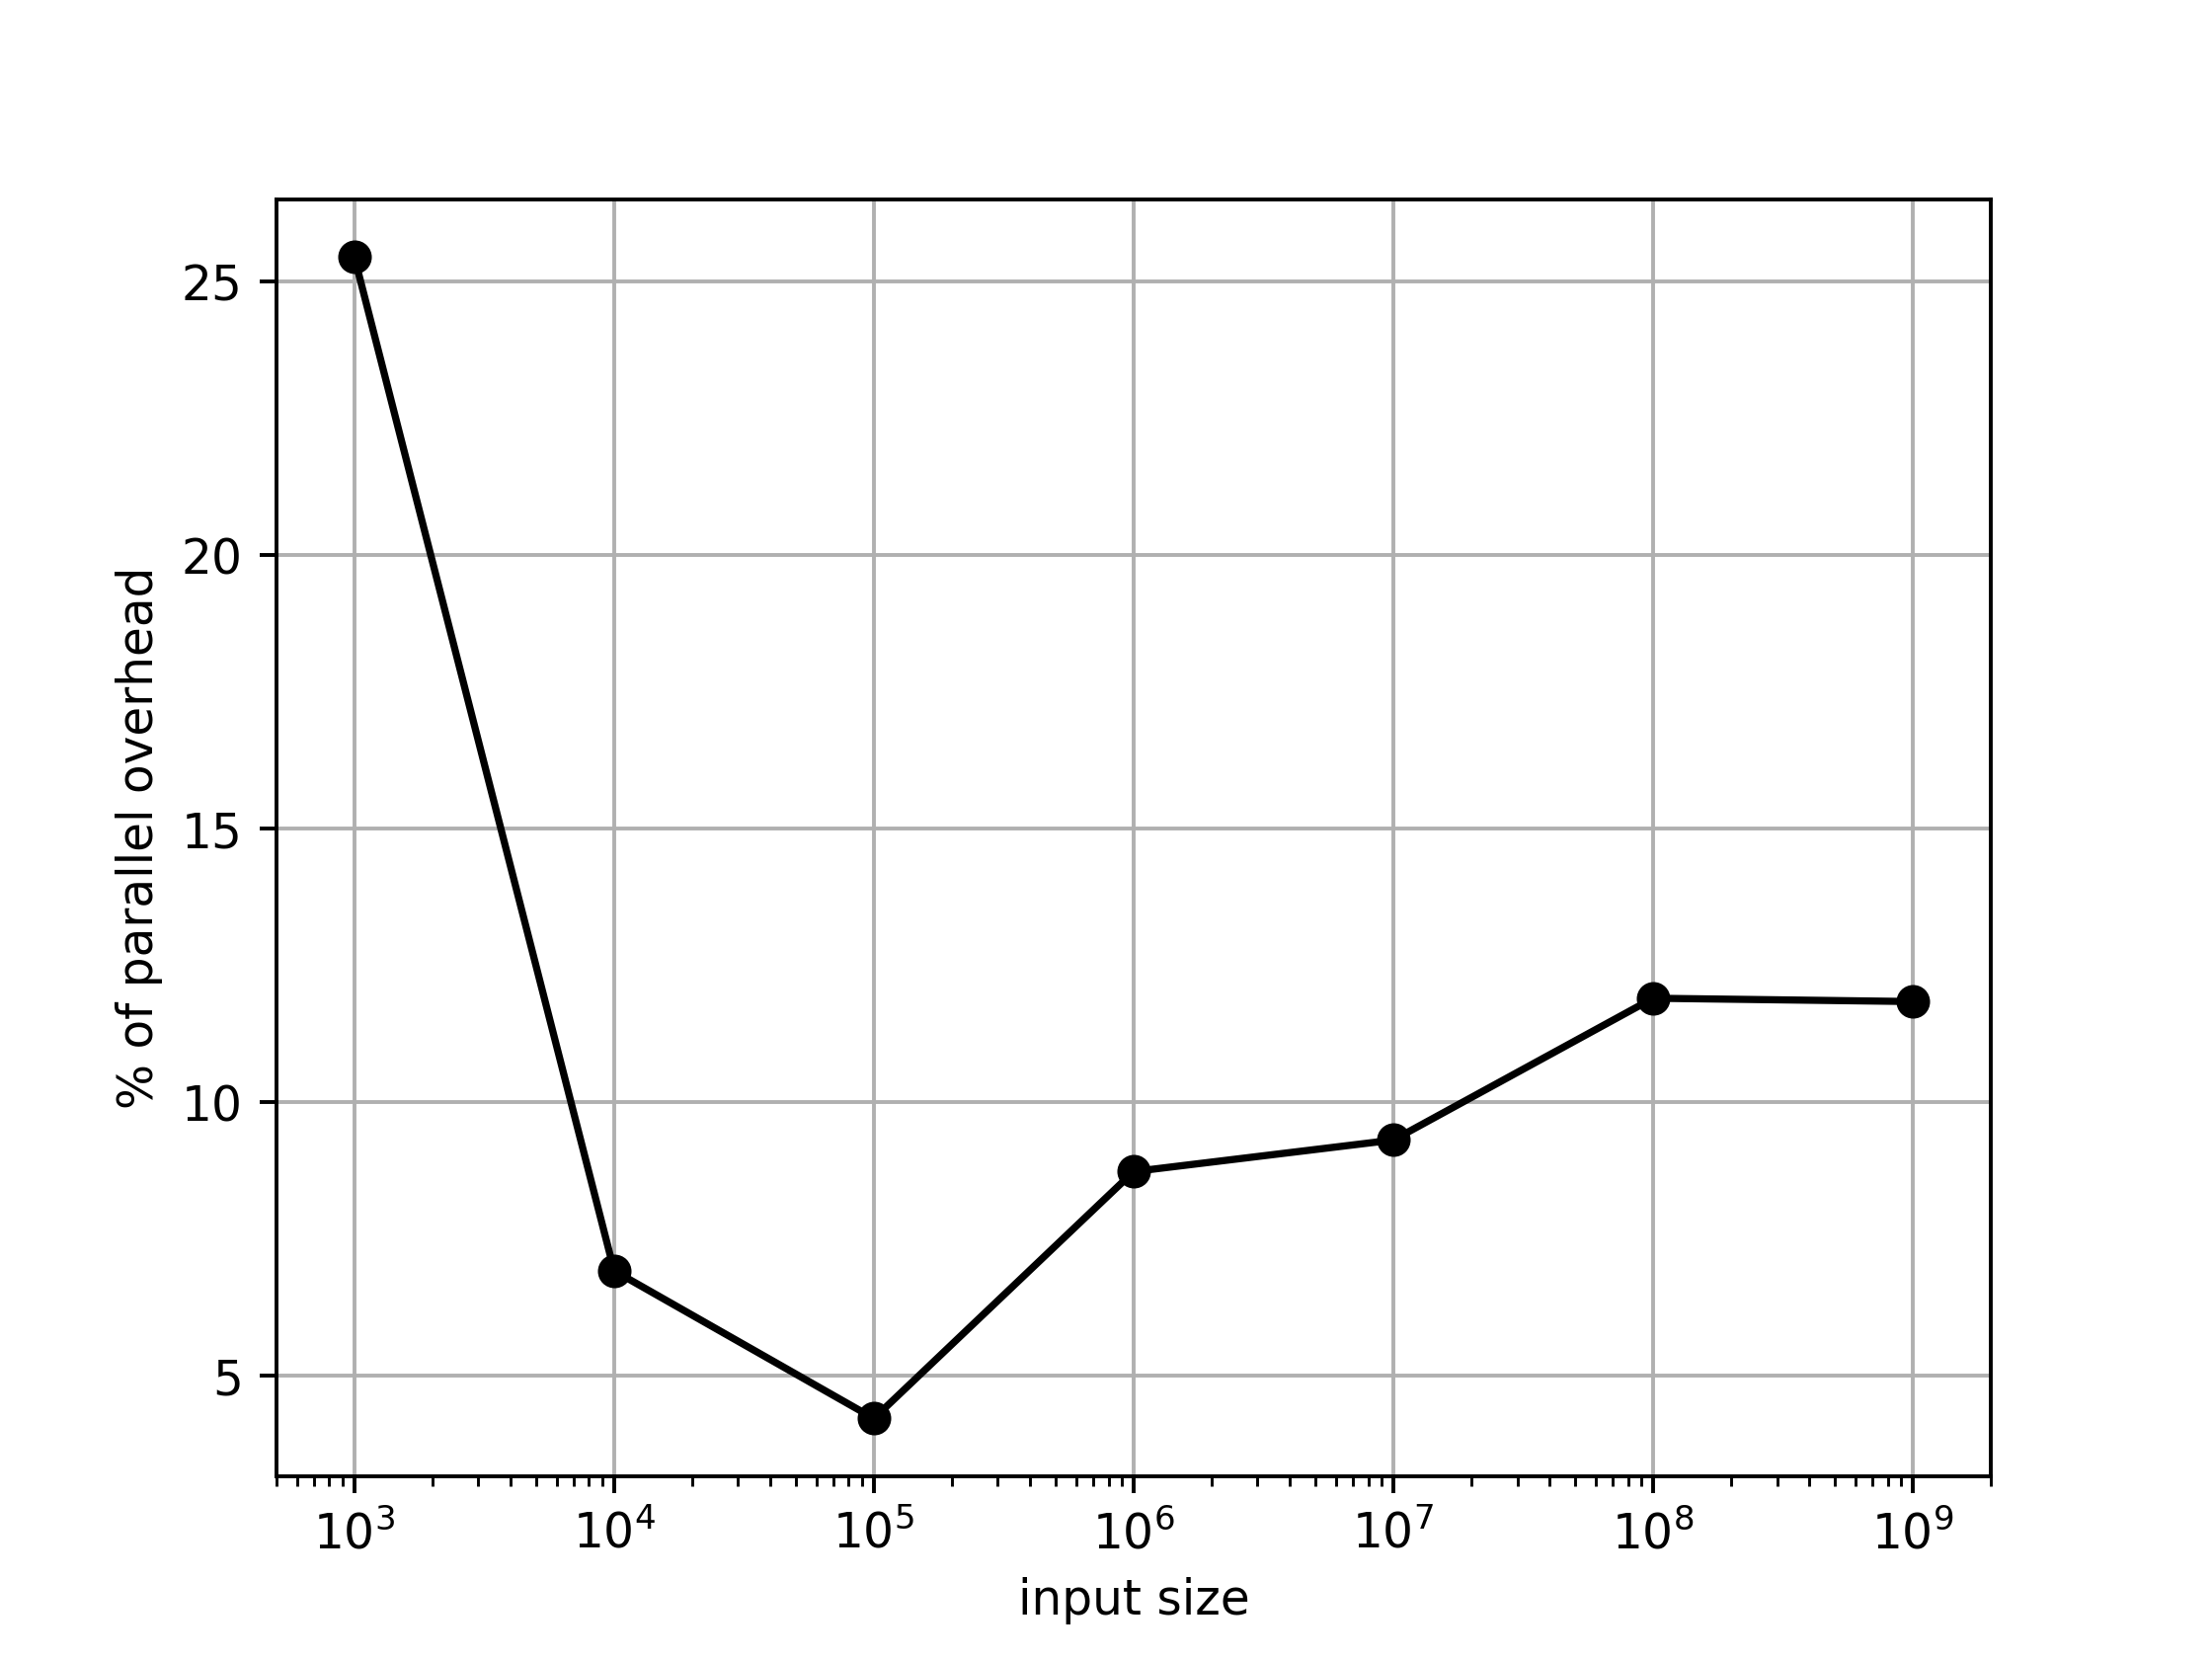
\includegraphics[width=\textwidth]{overhead.png}
        \caption{input size vs \% of parallel overhead}
        \label{fig:q1p1}
    \end{figure}
    We define overhead percentage $O$ as the percentage of difference between serial and parallel code execution time on 1 core with respect to the serial execution time.
    \begin{equation}
        O = \frac{T_{p_1} - T_s}{T_s} \cdot 100
    \end{equation}
    \textbf{Figure \ref{fig:q1p1}} shows the variation of the parallel overhead with input size. Parallel overhead is measured as \% of the serial time for the corresponding input size. We see that for a size of $10^3$ the overhead time by the parallel code is 25\%. As the problem size increases, this overhead decreases, with it being at about 5\% for input size $10^5$. After this it again starts increasing gradually, becoming about 12\% for input size $10^9$.
    
    For small input sizes, we see a greater overhead because for these problems, the actual compute time is very low, therefore the parallel overhead is a larger percentage of the serial time. Whereas, for larger problems, the compute time is very high and therefore the parallel overhead percentage is very low.
    \subsection{Input size vs execution time}
    \begin{figure}[H]
        \centering
        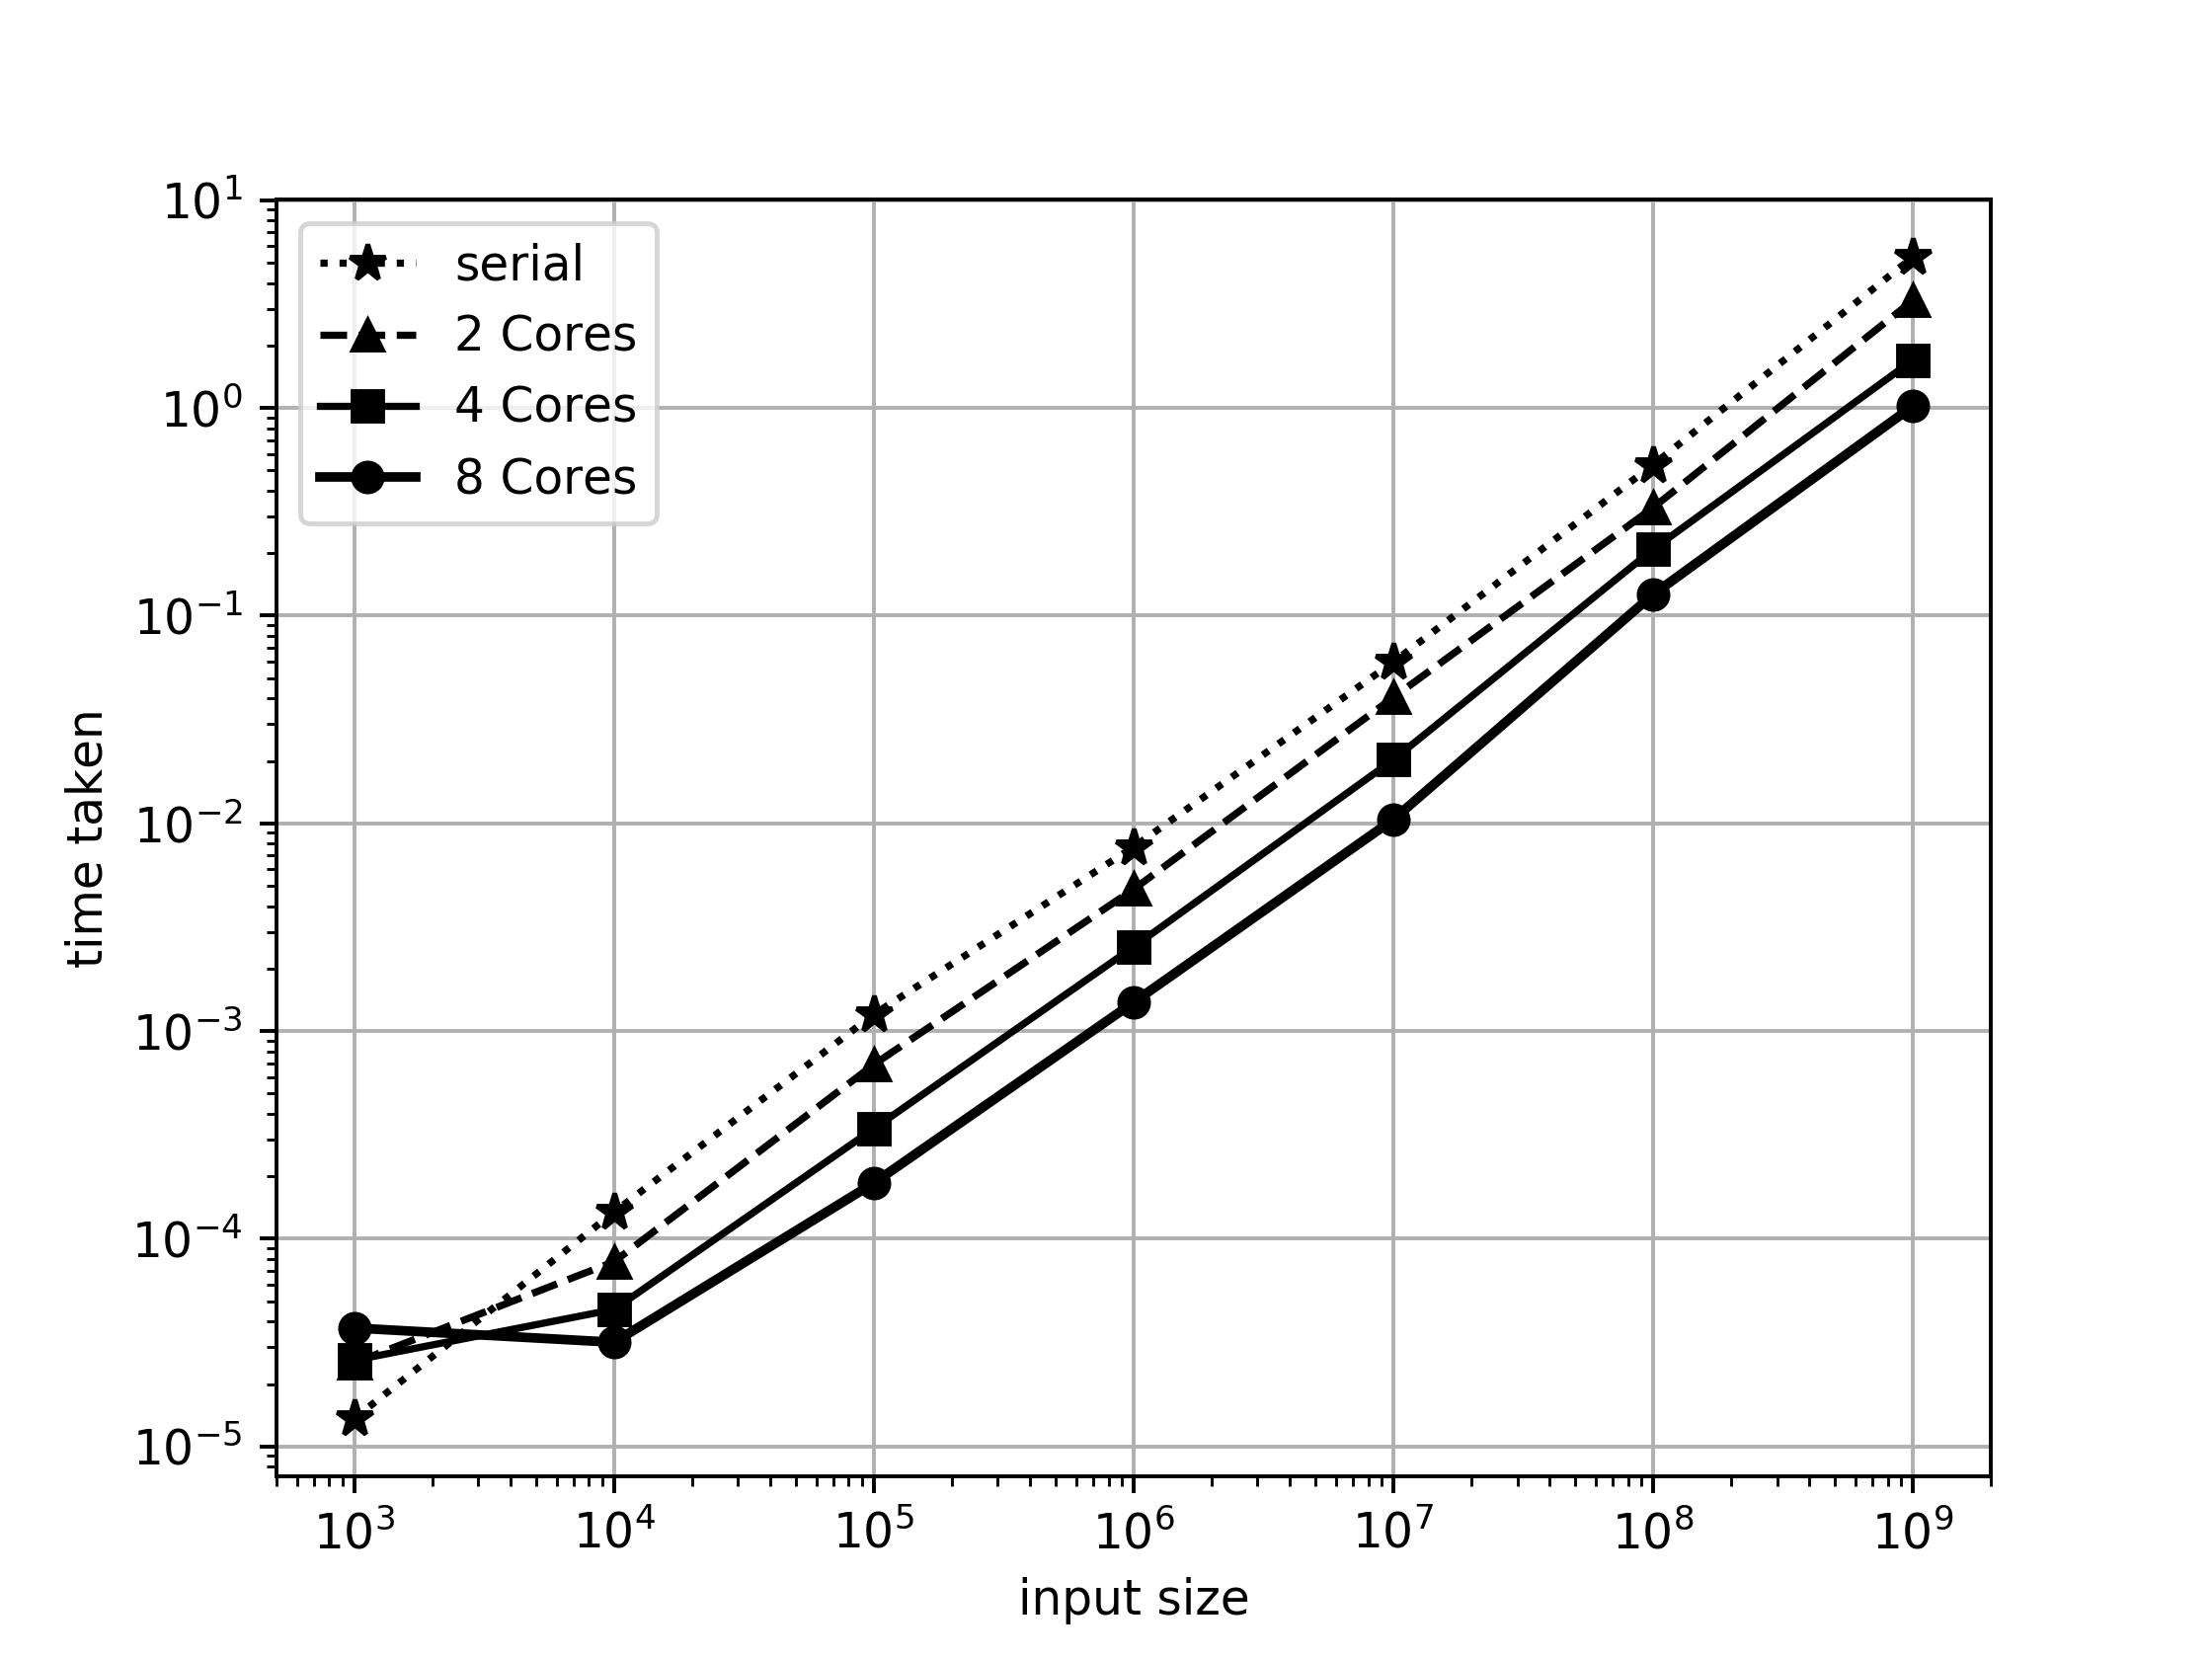
\includegraphics[width=\textwidth]{time.png}
        \caption{input size vs execution time in log-log scale}
        \label{fig:q1p2}
    \end{figure}
    As we increase the problem size by a factor of 10, we expect the execution time to also increase more or less proportionately. Off course this is a gross estimation which does not take into account the caching in the architecture. Also as we increase the number of cores, for a given input size, the execution time should decrease (for an optimal parallel algorithm). \textbf{Figure \ref{fig:q1p2}} is the actual curve we get from our experiments. Not that it is plotted in log-log scale considering the huge ranges of data.We see that this more or less adheres to our observations, with only one exception.
    
    For low input sizes, of the order of $10^3$, the execution time increases as we increase the number of cores. For small input sizes, the actual serial computation time is very low. Parallelizing the code only adds some more overheads, which dominate for small input sizes. The time taken for synchronization, and load distribution is greater than the time saved by parallelizing the code. Whereas, this is not the case for large input sizes, because here although the compute time increases significantly, the parallel overhead remains more or less the same.
    \newpage
    \subsection{Speedup vs input size}
    \begin{equation}
        speedup = \frac{T_{serial}}{T_{parallel}}
    \end{equation}
    \begin{figure}[H]
        \centering
        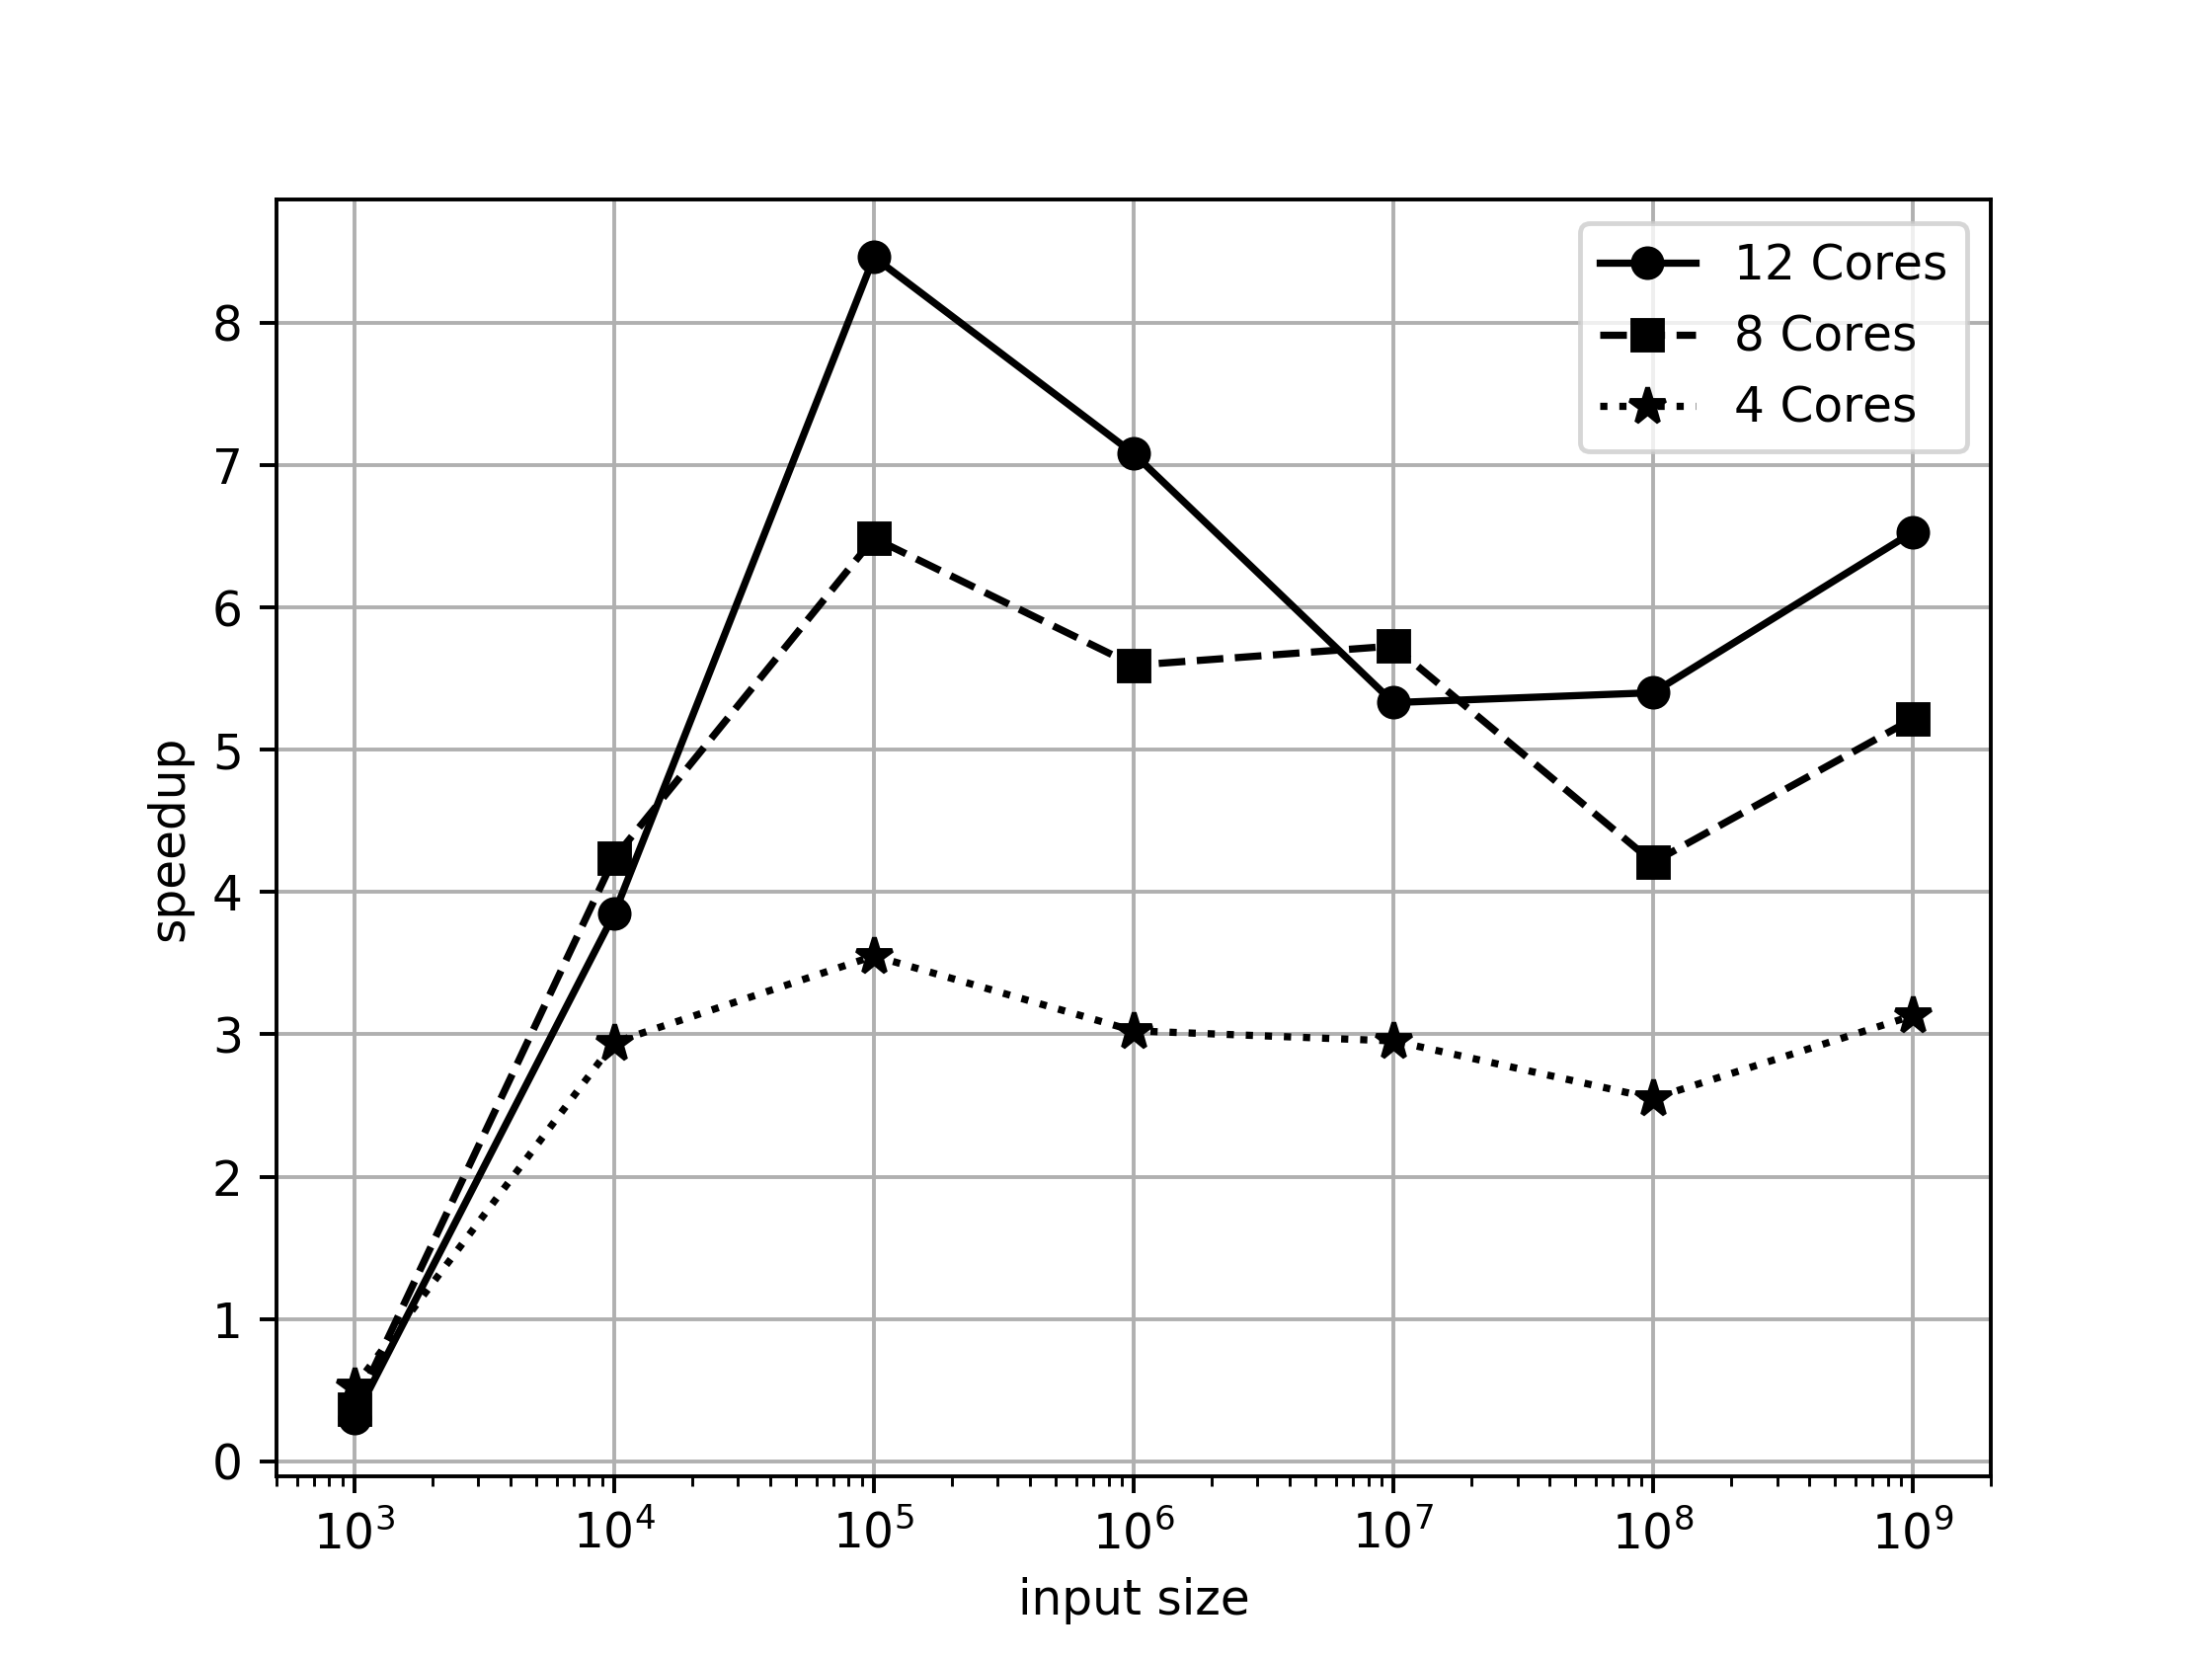
\includegraphics[width=\textwidth]{speedup_size.png}
        \caption{speedup vs input size}
        \label{fig:q1p3}
    \end{figure}
    \textbf{Figure \ref{fig:q1p3}} shows the variation of speedup with problem size. Notice that speedup first increases till problem size becomes $10^5$ and then starts decreasing till problem size becomes $10^8$. After this, it increases slightly till problem size becomes $10^9$. An important pattern emerges here. Notice that irrespective of the number of processors, speedup is maximum when input size is of the order of $10^5$.
    
    One possible reason for this might be the NUMA model which the computer follows. Initially as the input size is small, the parallel overhead dominates over the time saved by parallelizing the code. As the problem size increases, the compute time becomes larger , whereas the parallel overhead remains more or less the same. Hence more compute time is saved by parallelizing the code thereby giving us greater and greater speedup.
    
    After the array sizes becomes sufficiently large, each processor's cache cannot hold the array by itself. Therefore, it needs to access the array from the main memory, thereby increasing the time taken to compute.
    \subsection{Speedup vs number of cores}
    \begin{figure}[H]
        \centering
        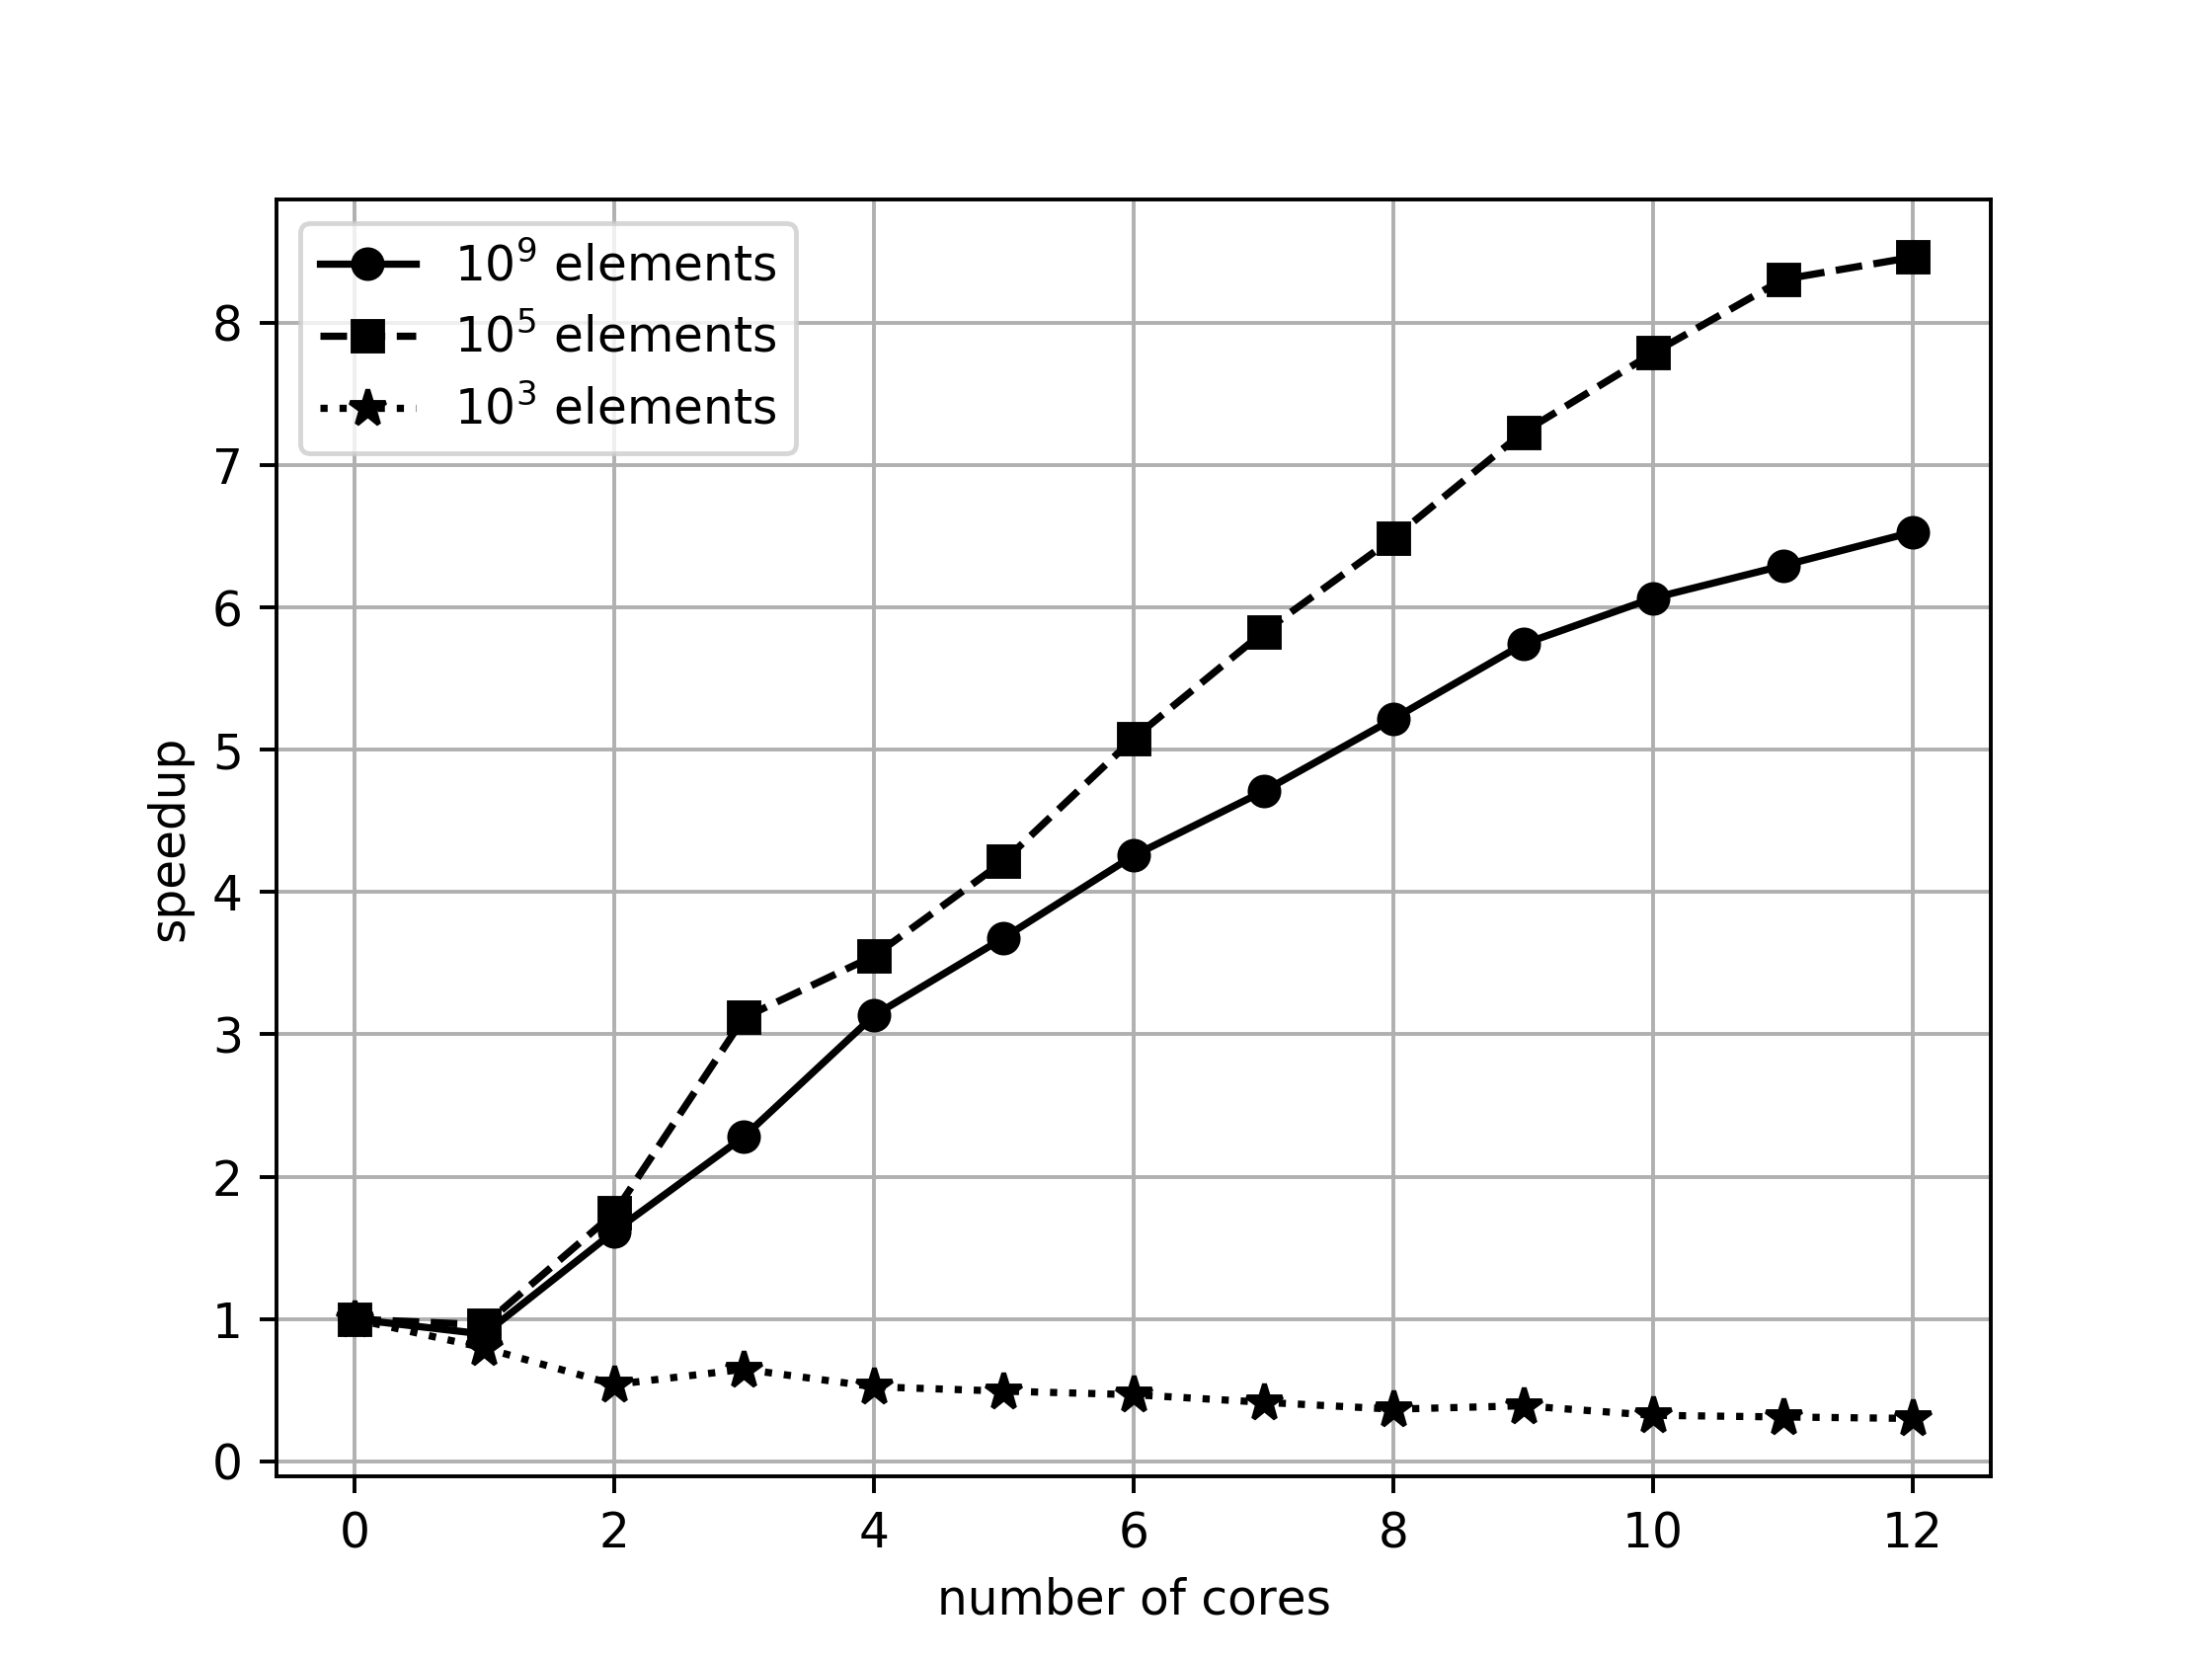
\includegraphics[width=\textwidth]{speedup_cores.png}
        \caption{speedup vs number of cores}
        \label{fig:q1p4}
    \end{figure}
    \textbf{Figure \ref{fig:q1p4}} shows the variation of speedup with the number of cores for different problem sizes. 2 notable patterns can be seen here.
    
    When the problem size is small(of the order of $10^3$), increasing the number of cores just adds more parallel overhead because of increased inter-processor synchronization and communication. This is not compensated by the time saved in parallelization since the compute time is already very low incase of the serial code.
    
    For large problem sizes, the case is opposite. Adding a new processor increases the speedup. This is because the compute time is inversely proportional to the number of processors. For large input sizes, the compute time is very high. So even though the parallel overhead increases slightly, a huge amount of time is saved by adding one extra processor. However note that the marginal gain in speedup by addition of 1 processor decreases as the number of processors increase. Thus speedup follows the \textbf{law of diminishing marginal returns
    
    \subsection{Efficiency Curve}
    \begin{figure}[H]
        \centering
        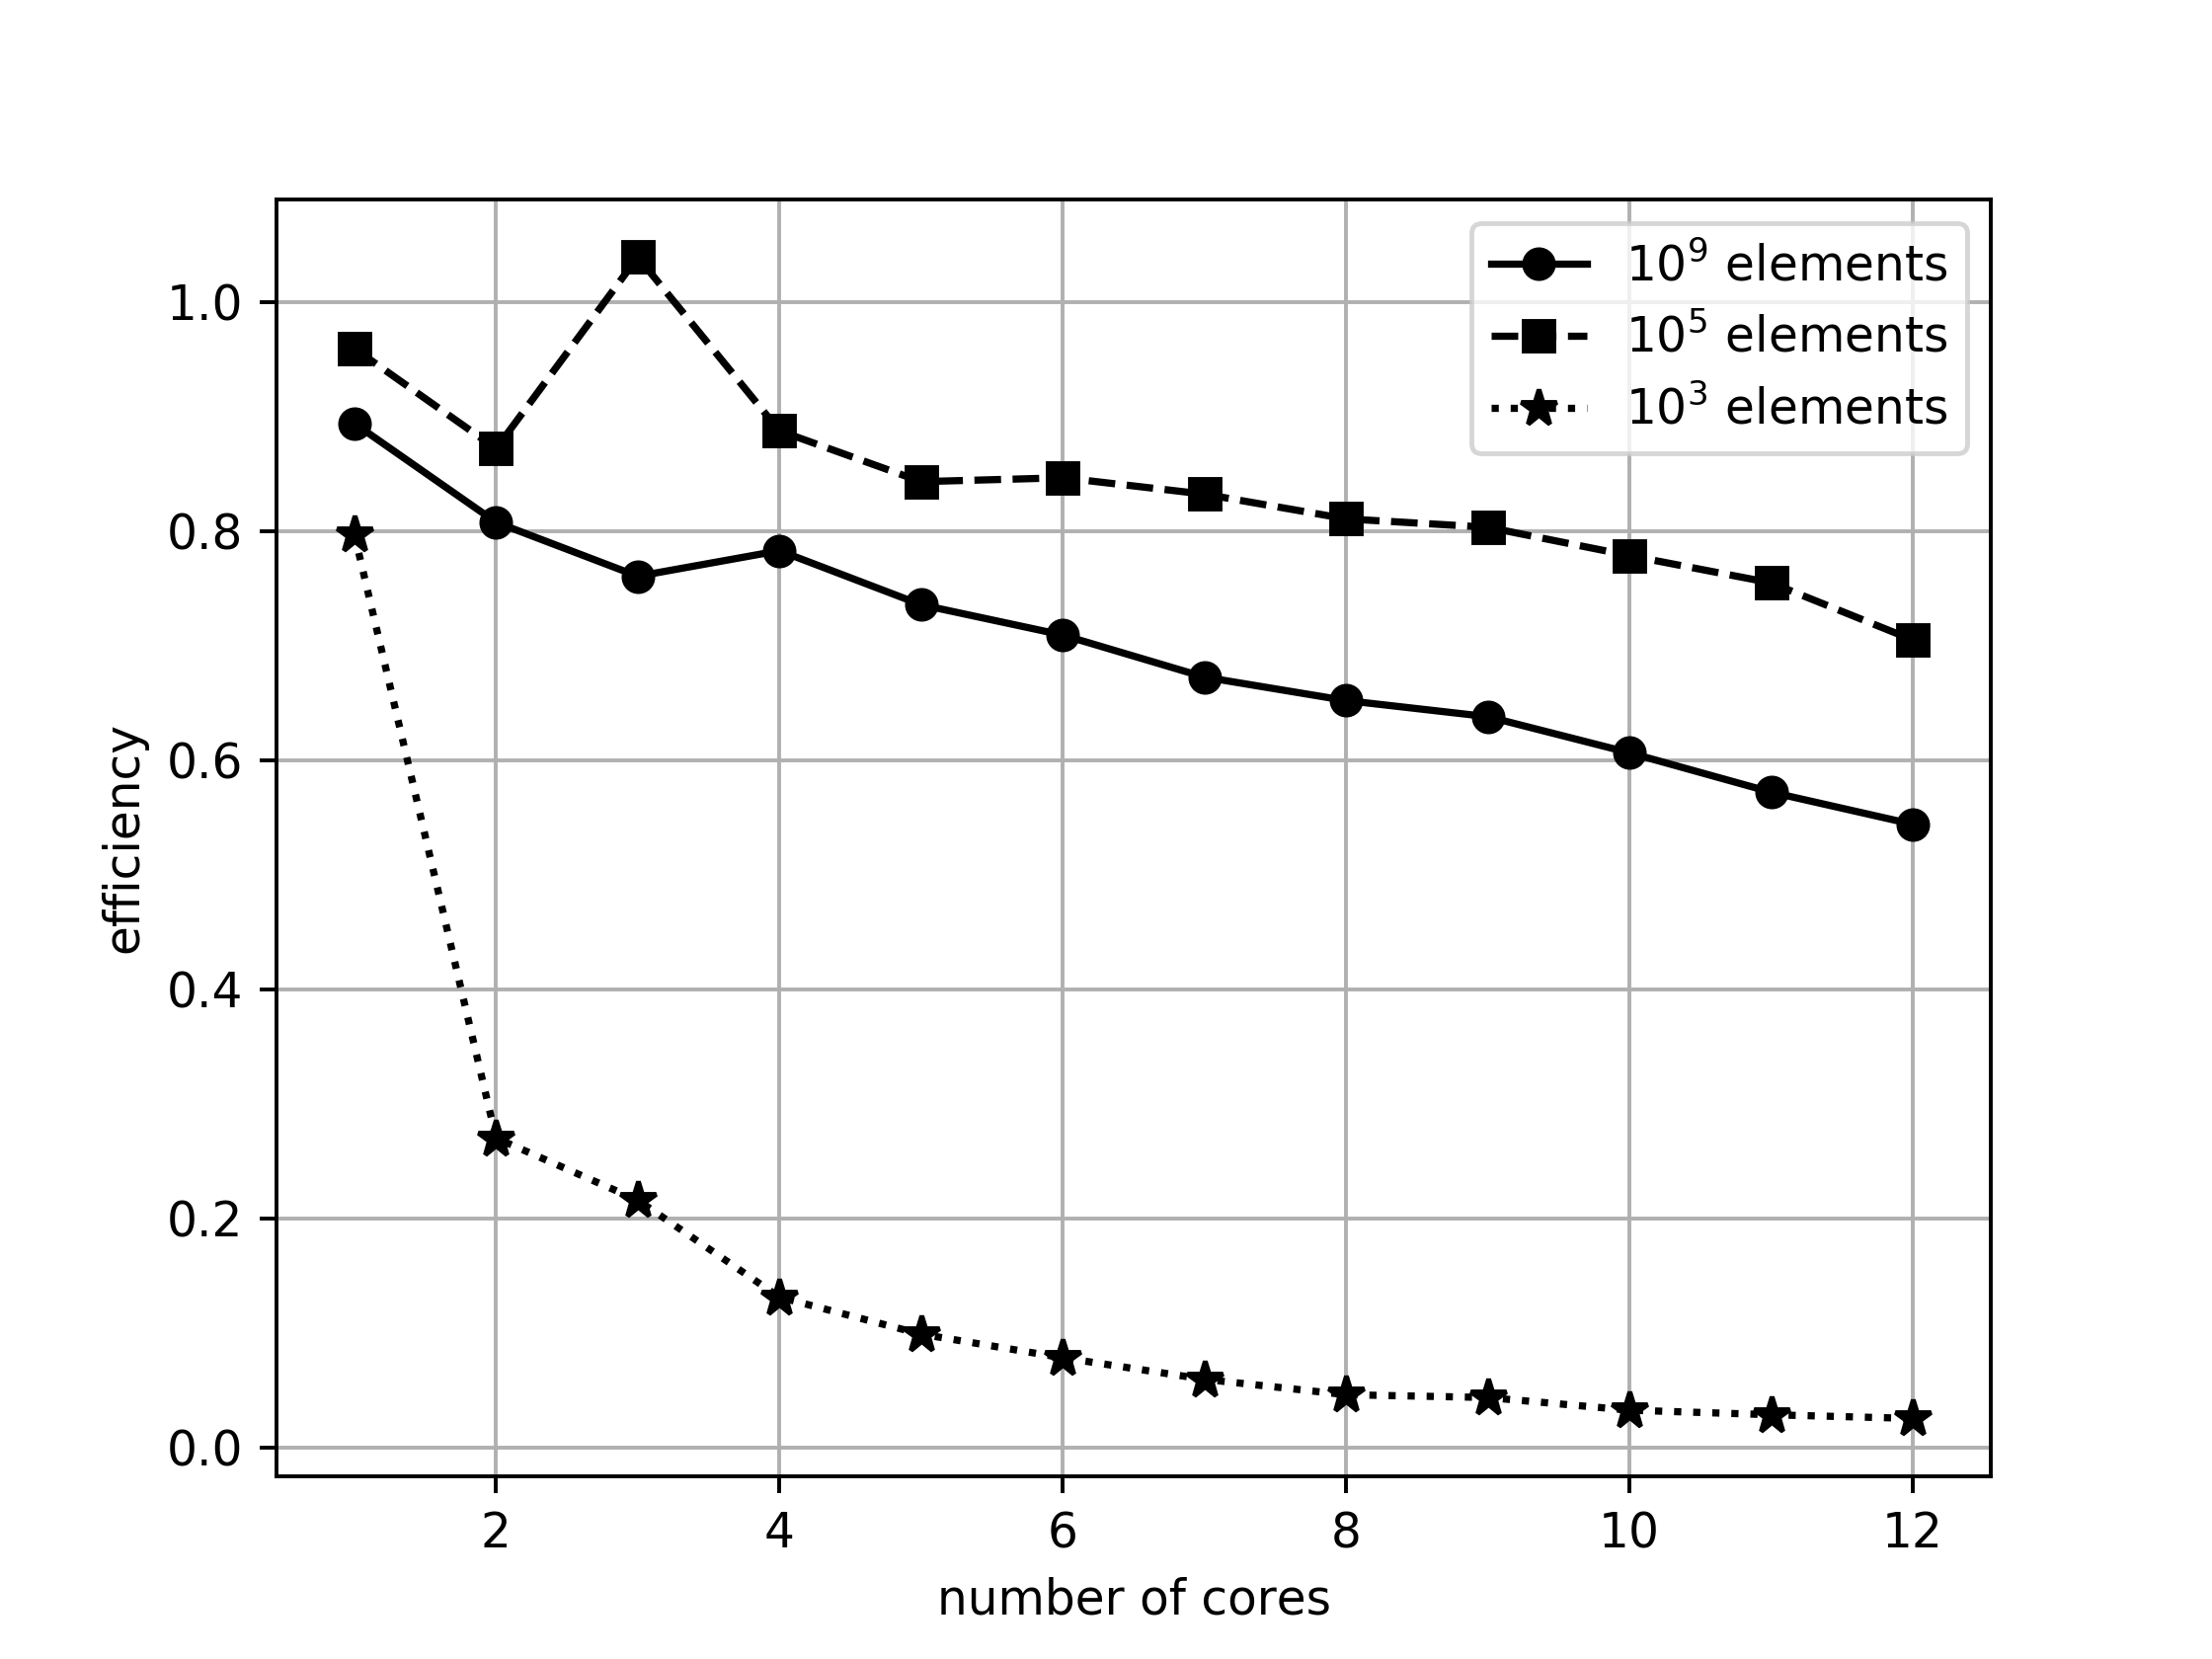
\includegraphics[width=\textwidth]{efficiency_cores.png}
        \caption{efficiency vs number of cores}
        \label{fig:q1p5}
    \end{figure}
    Efficiency $e$ is defined as speedup per unit processors. It is the ratio of $s_p$, the speedup in case of $p$ processors and $p$.
    \begin{equation}
        e = \frac{s_p}{p}
    \end{equation}
    As seen in the previous section, the speedup follows the law of diminishing marginal returns in this problem. Therefore when we plot the efficiency vs the number of cores, we expect a decreasing behavior. This argument is validated in \textbf{figure \ref{fig:q1p5}}.
    
    \emph{ A system whose performance improves after adding hardware, proportionally to the capacity added, is said to be a scalable system.}
    
    The efficiency decreases with increase in number of cores, hence this is a \textbf{weakly scalable}. One possible reason for this might be the fact that the load might not get equally distributed across all processors. Another reason might be that all the processors are accessing the same memory i.e. array in this case. Hence the access speed decreases as a lot of processors try to fetch the array elements, thereby further decreasing the speedup.
    
    \section{Calculation of $\pi$ : Monte Carlo method}
    
    The Monte Carlo method is a stochastic method which can be used to calculate the value of $\pi$.
    \begin{figure}[H]
        \centering
        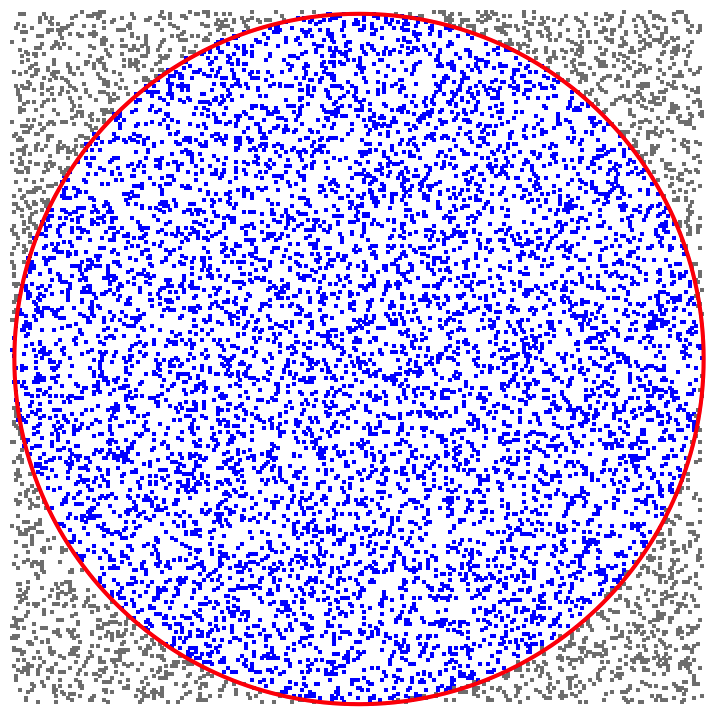
\includegraphics[width=0.5\textwidth]{UgAd4.png}
        \caption{Monte Carlo method for the calculation of $\pi$}
        \label{fig:my_label}
    \end{figure}
    Basically in this method, random "darts" are projected in a 2x2 square space. Let number of darts projected on the circular region be $n_c$. Let total number of points be $N$. Therefore the probability of a random dart landing on the central circular region is $\frac{n_c}{N}$. Also the same probability is equal to $\frac{A_c}{A_s}$ where $A_c$ is the area of the circle and $A_s$ is the area of square. $A_c$ has the value $\pi$ since the radius of the circle is 1 and $A_s$ has the value 4. Therefore:
    \begin{equation}
        \frac{\pi}{4} = \frac{n_c}{N}
    \end{equation}
    The following is the serial implementation of the algorithm in C++14:
    \begin{lstlisting}
        double getPi(long numPoints) {
            long n_c = 0;
            for(int i=0;i<numPoints;i++) {
                double x = -1 + (2.0*rand())/(RAND_MAX);
                double y = -1 + (2.0*rand())/(RAND_MAX);
                if(sqrt(x*x + y*y)<=1)
                    n_c++;
            }
            double pi = (4.0*n_c)/(num*1.0);
            return(pi);
        }
    \end{lstlisting}
    Notice that we are using the \code{rand()} function in the serial implementation.
    \subsection{Parallelizing the serial code}
    If we take a close look at the serial code, we see that the output is just summation on \code{n\_c}. A naive approach would be to parallelize the for loop amongst various threads by using \code{omp parallel for} directive with the summation on \code{n\_c} done as a \textbf{critical} or an \textbf{atomic} operation by using \code{omp critical} or \code{omp atomic} directives respectively.
    
    However, the introduction of critical or atomic regions will degrade the performance, because only one thread can access the critical section of the code. A better solution would be to apply \textbf{reduction}. We can apply reduction here because summation(+) is an associative  and a commutative operation. We apply reduction using the \code{omp reduction(+:n\_c)} clause along with the \code{omp parallel for} directive. The following is the initial implementation of the code in C++14:
    \begin{lstlisting}
    double getPi(long numPoints) {
            long n_c = 0;
            #pragma omp parallel for reduction(+:n_c)
            for(int i=0;i<numPoints;i++) {
                double x = -1 + (2.0*rand())/(RAND_MAX);
                double y = -1 + (2.0*rand())/(RAND_MAX);
                if(sqrt(x*x + y*y)<=1)
                    n_c++;
            }
            double pi = (4.0*n_c)/(num*1.0);
            return(pi);
        }
    \end{lstlisting}
    However we encounter a problem. This code takes a much greater execution time as compared to even the naive serial code. This is because the function $rand()$ is not thread safe.
    \subsubsection{\code{rand()}}
    This function returns a random number from 0 to \code{RAND\_MAX}. It is a \textbf{linear congruential generator} which uses the following algorithm:
    \begin{equation}
        X_n+1 = (aX_n+c) mod m
    \end{equation}
    The value $X_n$ is saved as the state of the generator for the next use. THe problem with \code{rand()} is that its a non reentrant function i.e. entering into the function every time changes the state it has. Basically whenever a thread uses the \code{rand()} function, it modifies the state. To avoid multthreaded ace conditions, this step is made critical, thereby making it act as a bottleneck in the parallel code.
    \subsection{\code{rand\_r()}}
    This function is just a modification of the \code{rand()} function. We just pass the state as an integer pointer during function call, making it a thread safe method, since each thread can use a different seed.
    Thus the most optimal parallel code is :
    \begin{lstlisting}
    double getPi(long numPoints) {
            long n_c = 0;
            #pragma omp parallel{
                int seed = time(NULL)
                #pragma omp for reduction(+:n_c)
                for(int i=0;i<numPoints;i++) {
                    double x = -1 + (2.0*rand())/(RAND_MAX);
                    double y = -1 + (2.0*rand())/(RAND_MAX);
                    if(sqrt(x*x + y*y)<=1)
                        n_c++;
                }
            }
            double pi = (4.0*n_c)/(num*1.0);
            return(pi);
        }
    \end{lstlisting}
    \begin{figure}[H]
        \centering
        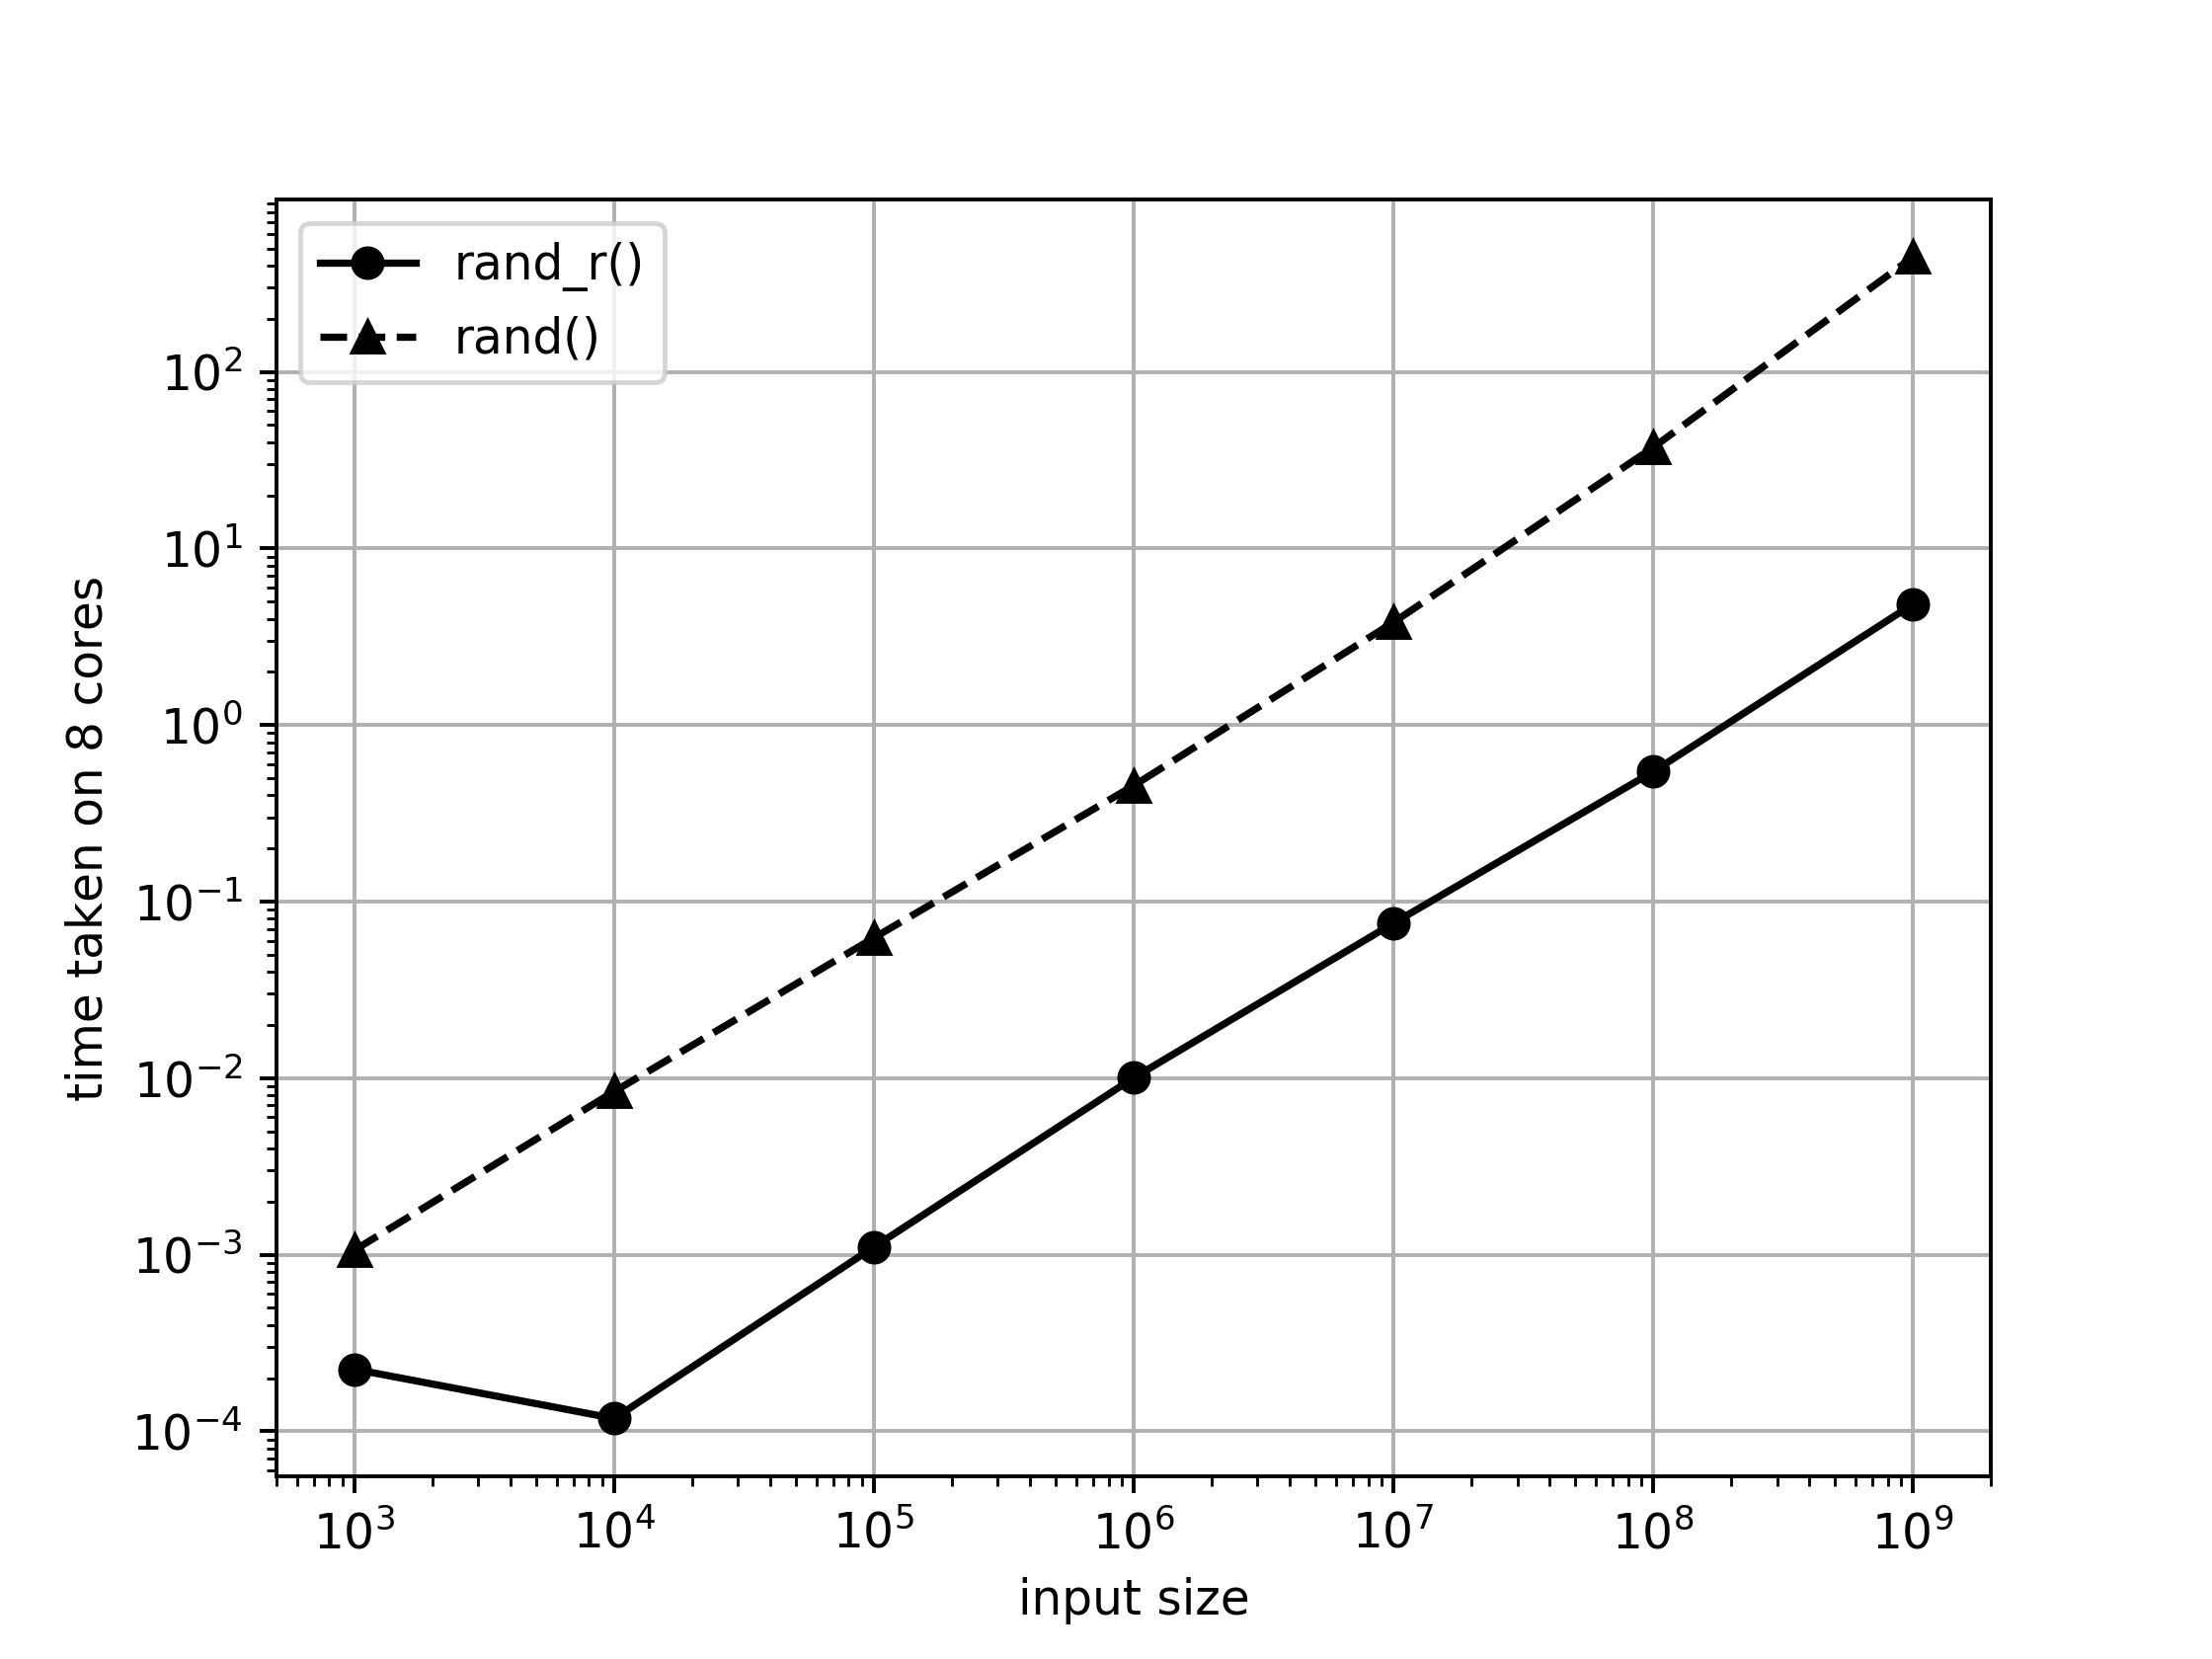
\includegraphics[width=\textwidth]{rand_rand_r.png}
        \caption{Time taken by rand vs rand\_r (log log scale)}
        \label{fig:q1p7}
    \end{figure}
    \subsection{Parallel overheads}
    We define overhead percentage $O$ as the percentage of difference between serial and parallel code execution time on 1 core with respect to the serial execution time.
    \begin{equation}
        O = \frac{T_{p_1} - T_s}{T_s} \cdot 100
    \end{equation}
    \begin{figure}[H]
        \centering
        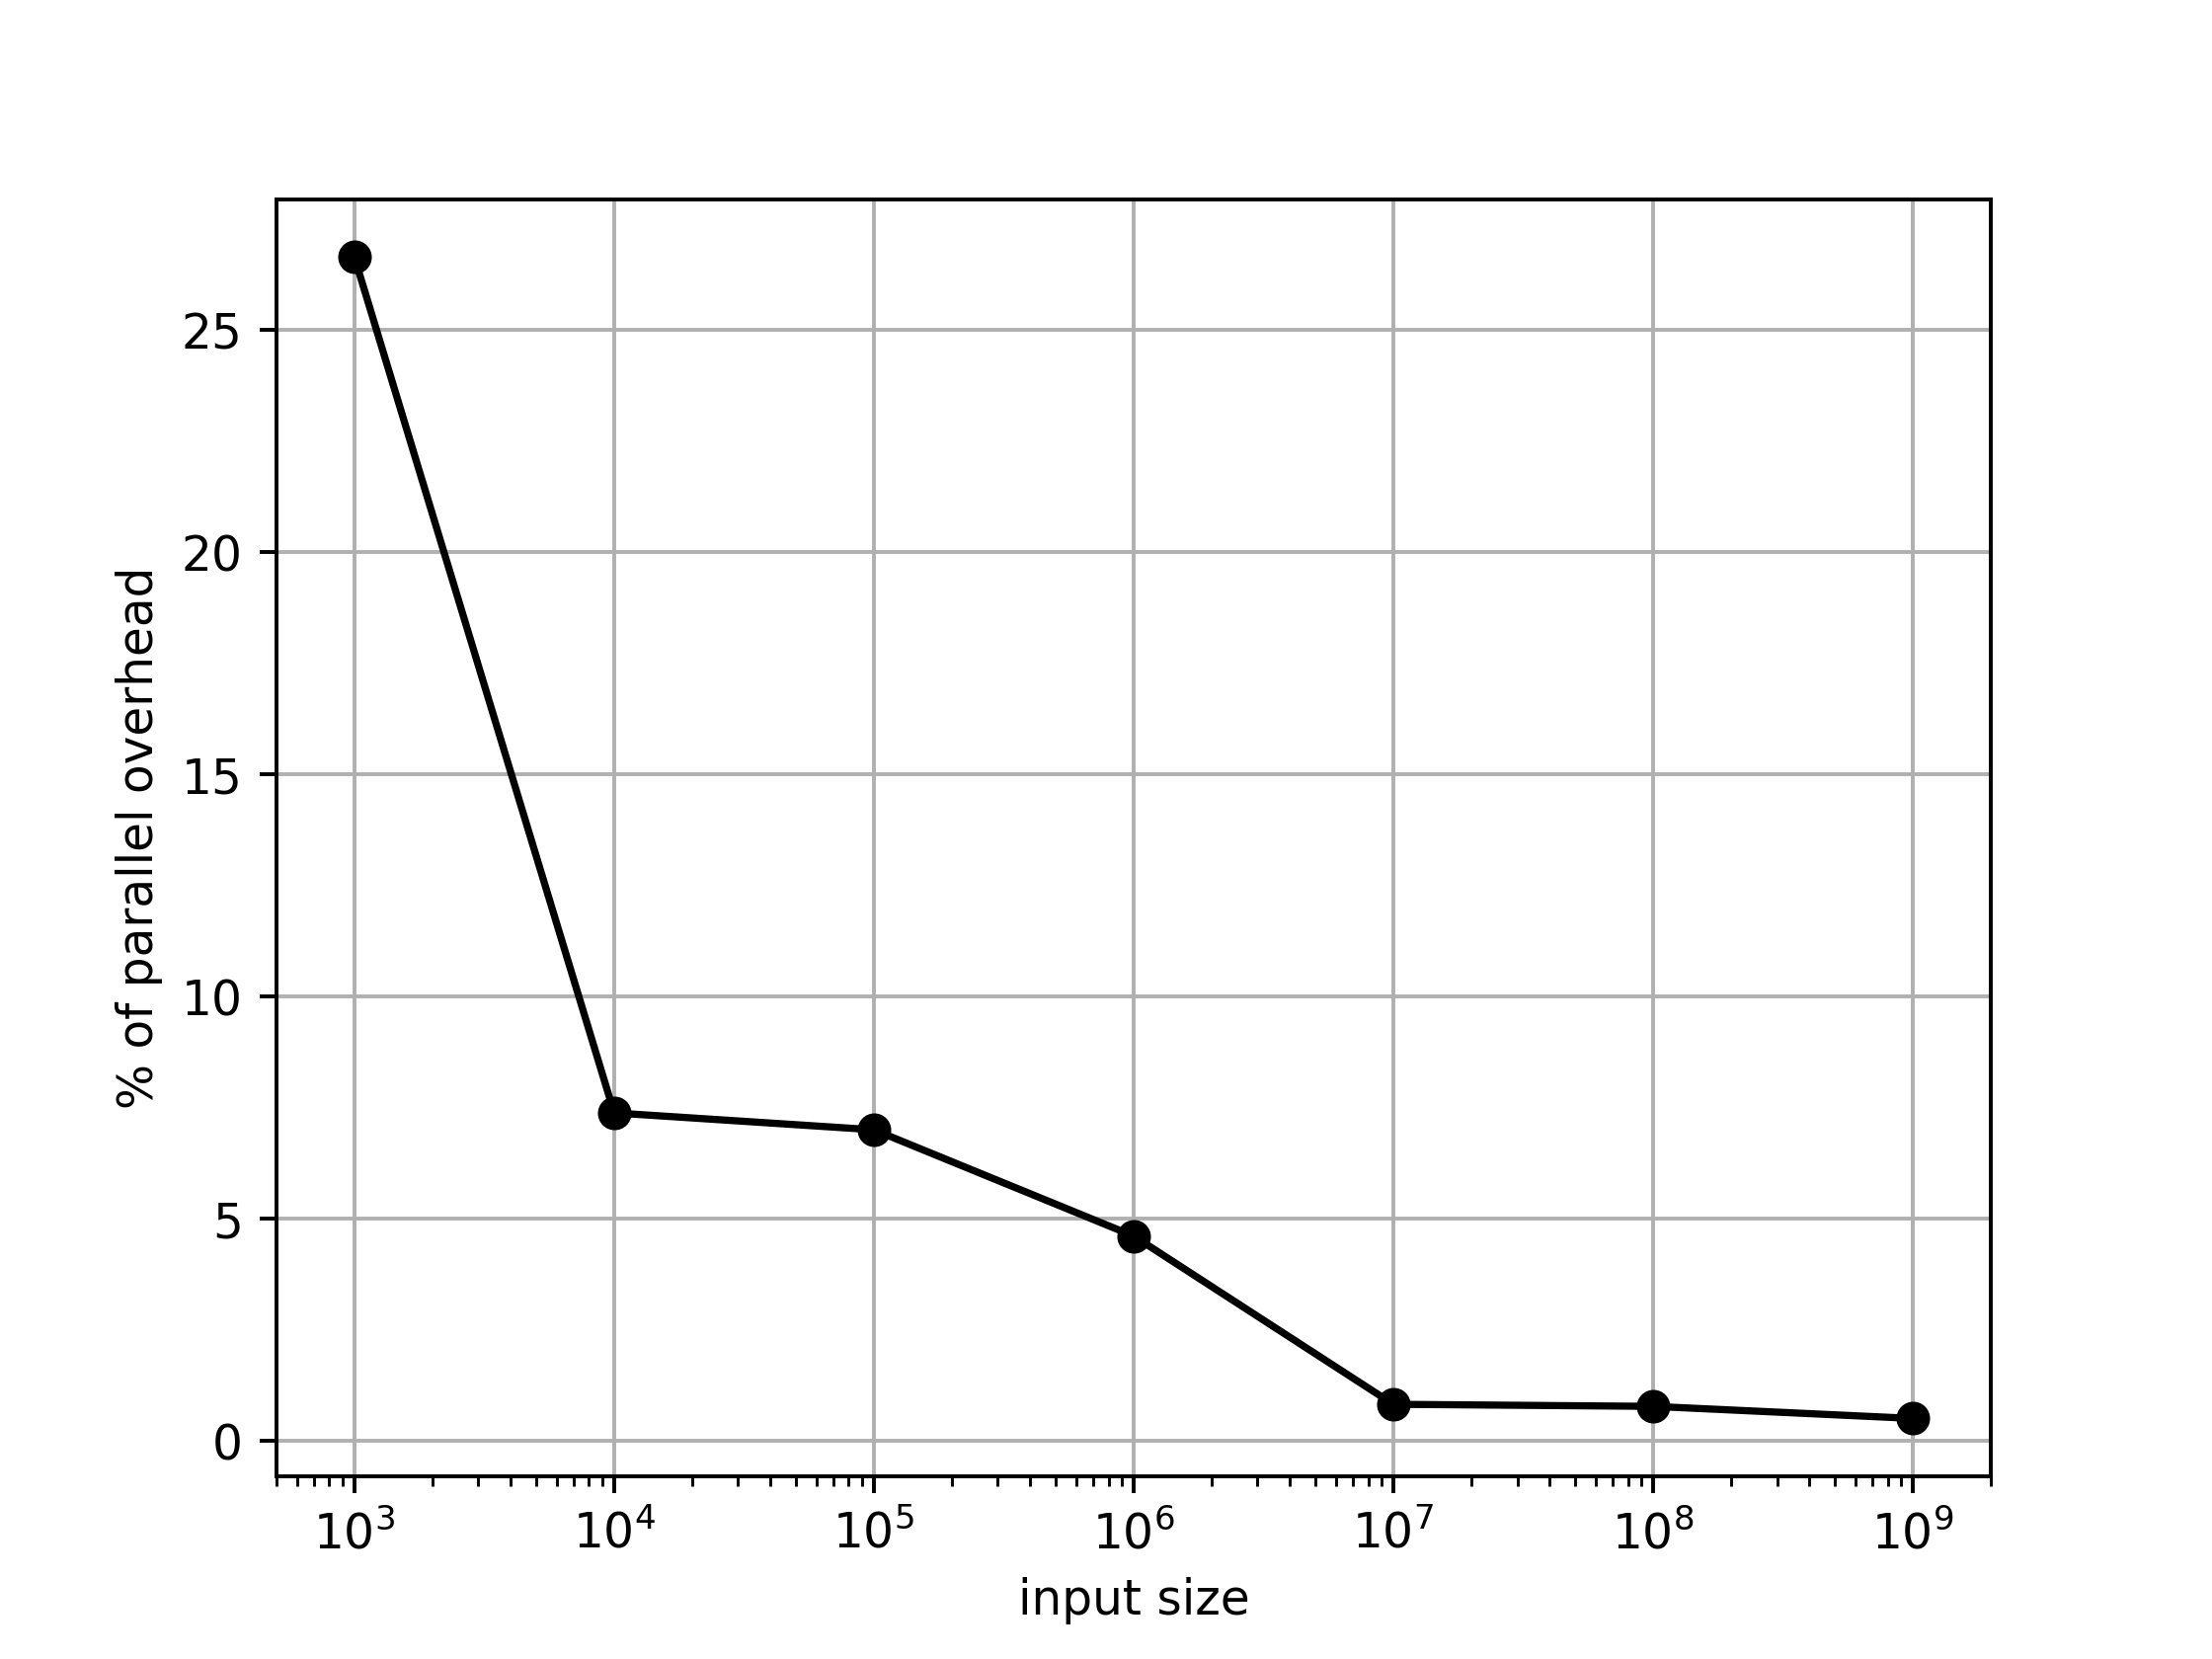
\includegraphics[width=\textwidth]{pioverhead.png}
        \caption{Parallel overhead vs input size}
        \label{fig:q1p8}
    \end{figure}
    In the above figure we see variation of parallel overhead with respect to the input size.
    
    For small input sizes, we see a greater overhead because for these problems, the actual compute time is very low, therefore the parallel overhead is a larger percentage of the serial time. Whereas, for larger problems, the compute time is very high and therefore the parallel overhead percentage is very low.
    
    For large input sizes the overhead is barely 2\%, whereas for very small inputs it can be as large as 25\%.
    \newpage
    \subsection{Input size vs execution time}
    \begin{figure}[H]
        \centering
        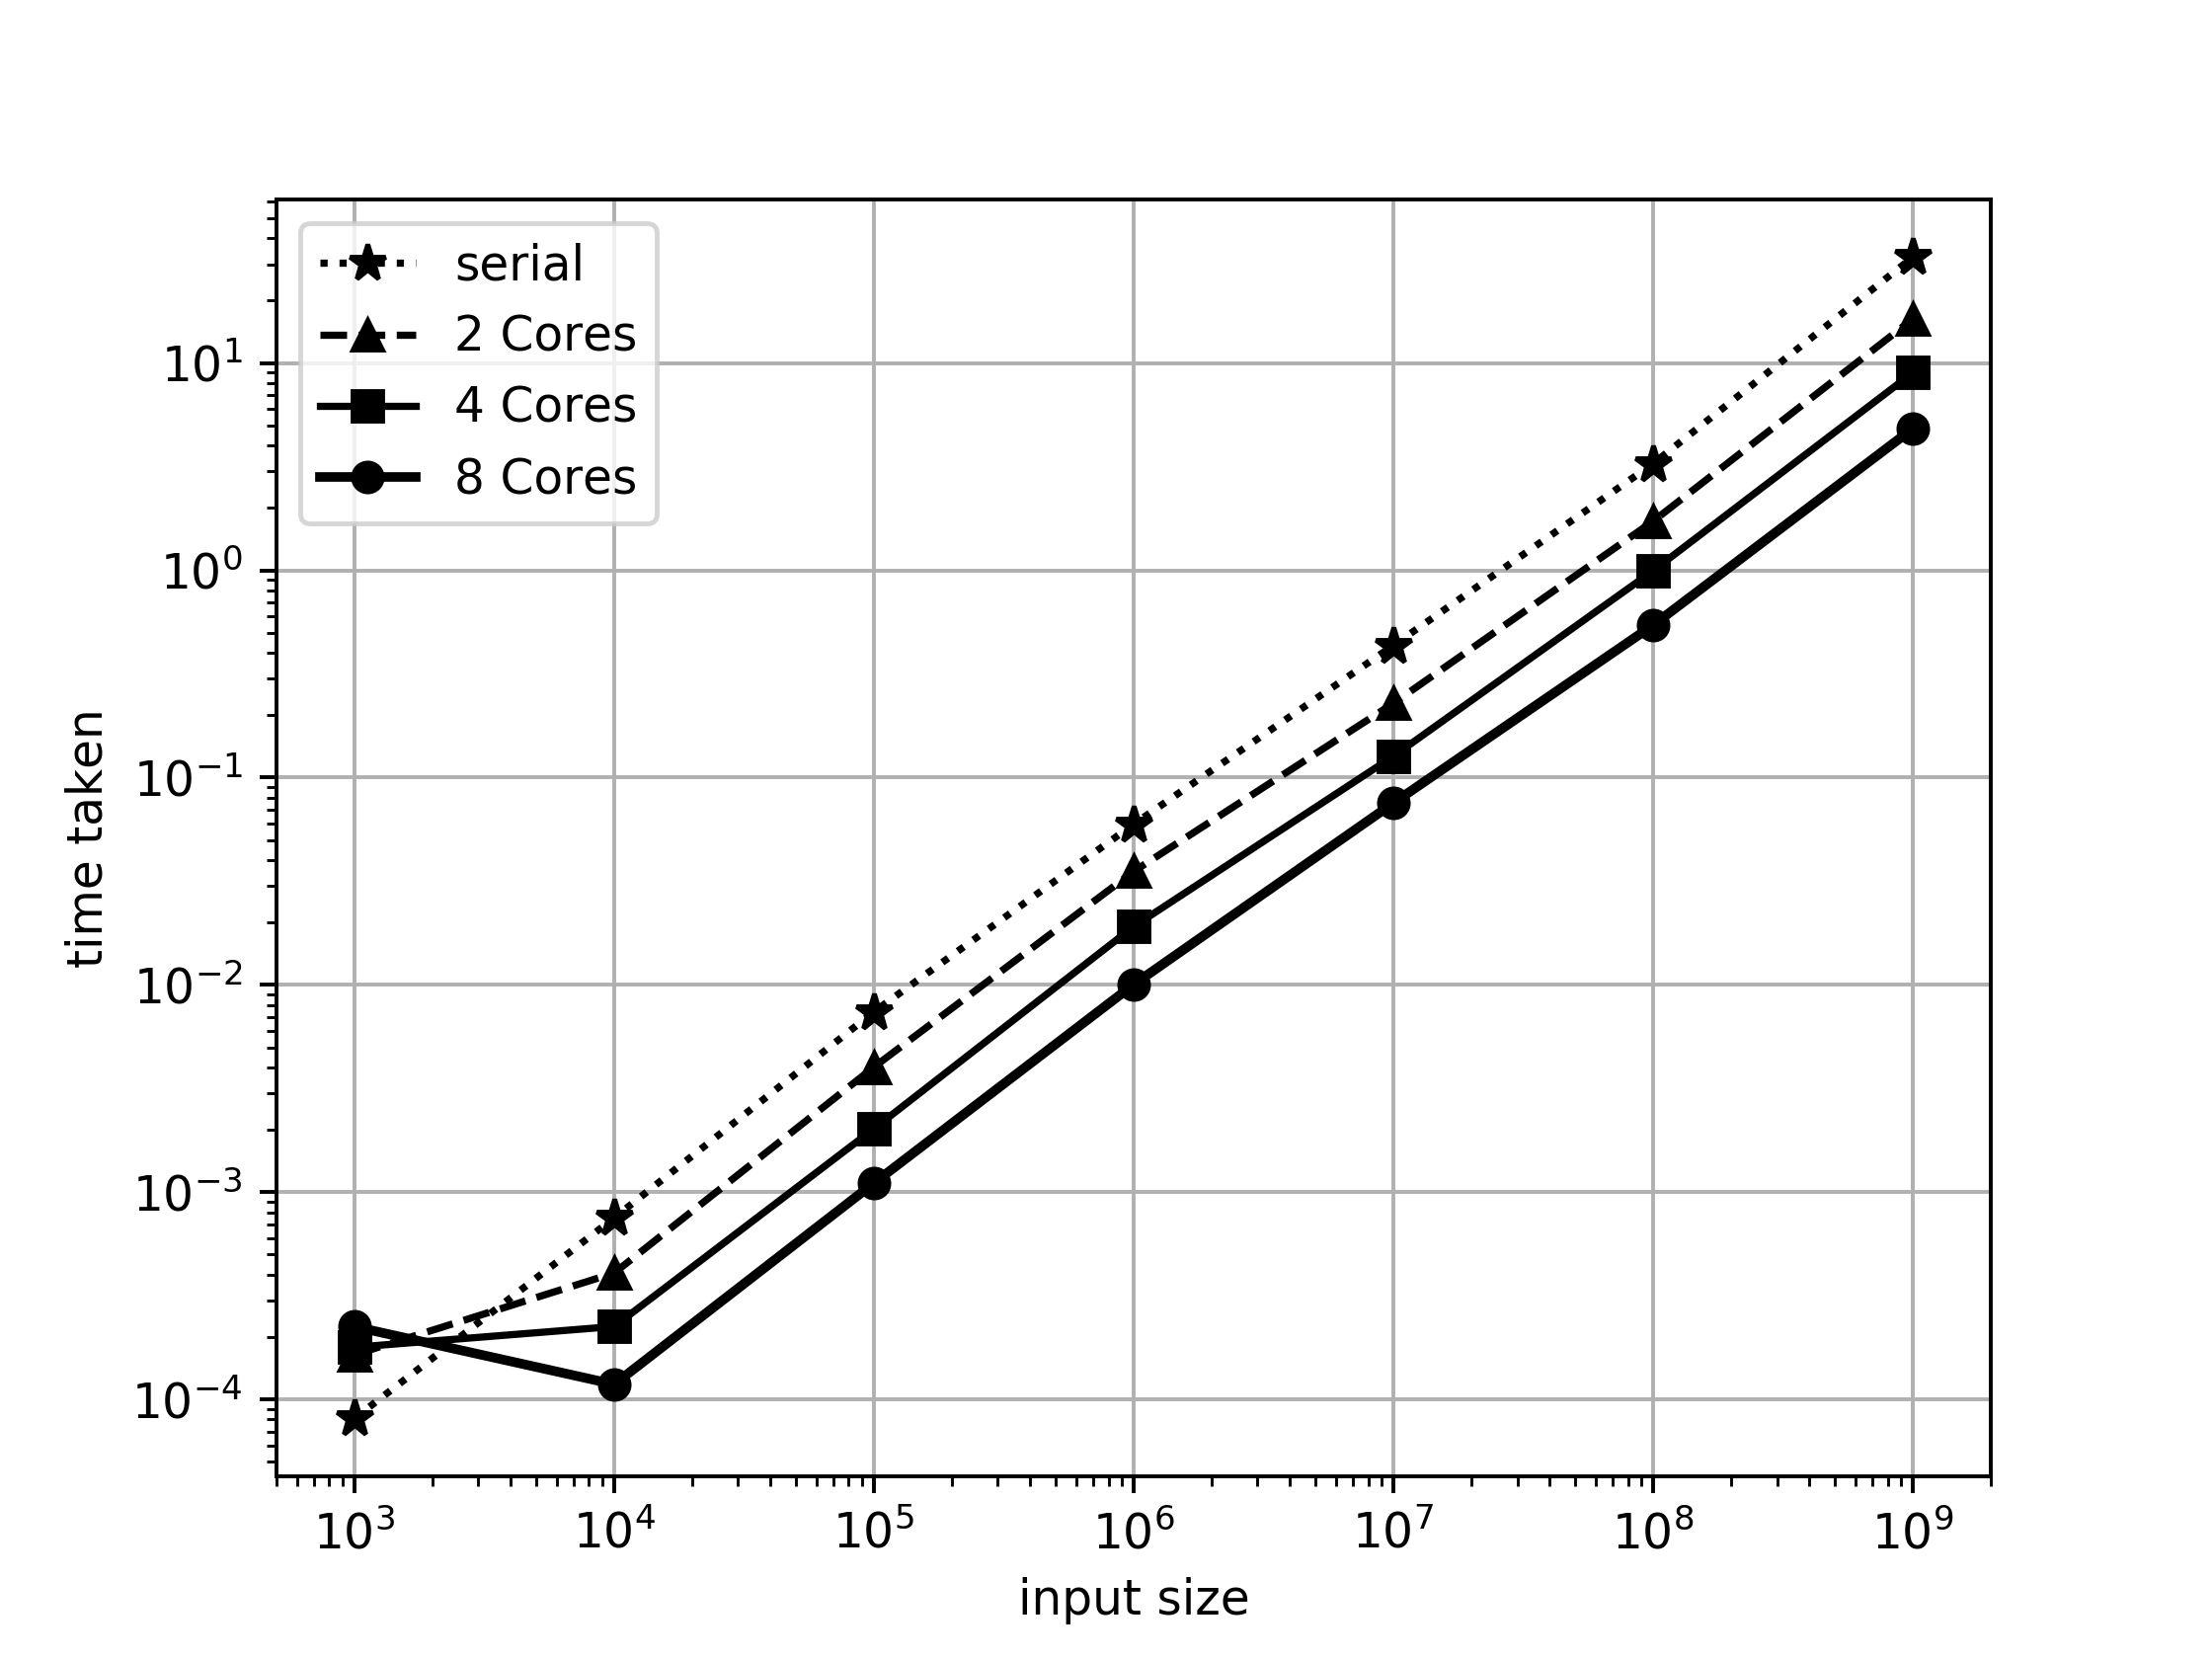
\includegraphics[width=\textwidth]{pitime.png}
        \caption{input size vs execution time}
        \label{fig:q1p9}
    \end{figure}
    As we increase the problem size by a factor of 10, we expect the execution time to also increase more or less proportionately. Off course this is a gross estimation which does not take into account the caching in the architecture. Also as we increase the number of cores, for a given input size, the execution time should decrease (for an optimal parallel algorithm). \textbf{Figure \ref{fig:q1p9}} is the actual curve we get from our experiments. Not that it is plotted in log-log scale considering the huge ranges of data.We see that this more or less adheres to our observations, with only one exception.
    
    For low input sizes, of the order of $10^3$, the execution time increases as we increase the number of cores. For small input sizes, the actual serial computation time is very low. Parallelizing the code only adds some more overheads, which dominate for small input sizes. The time taken for synchronization, and load distribution is greater than the time saved by parallelizing the code. Whereas, this is not the case for large input sizes, because here although the compute time increases significantly, the parallel overhead remains more or less the same.
    \newpage
    \subsection{Speedup vs input size}
    \begin{equation}
        speedup = \frac{T_{serial}}{T_{parallel}}
    \end{equation}
    \begin{figure}[H]
        \centering
        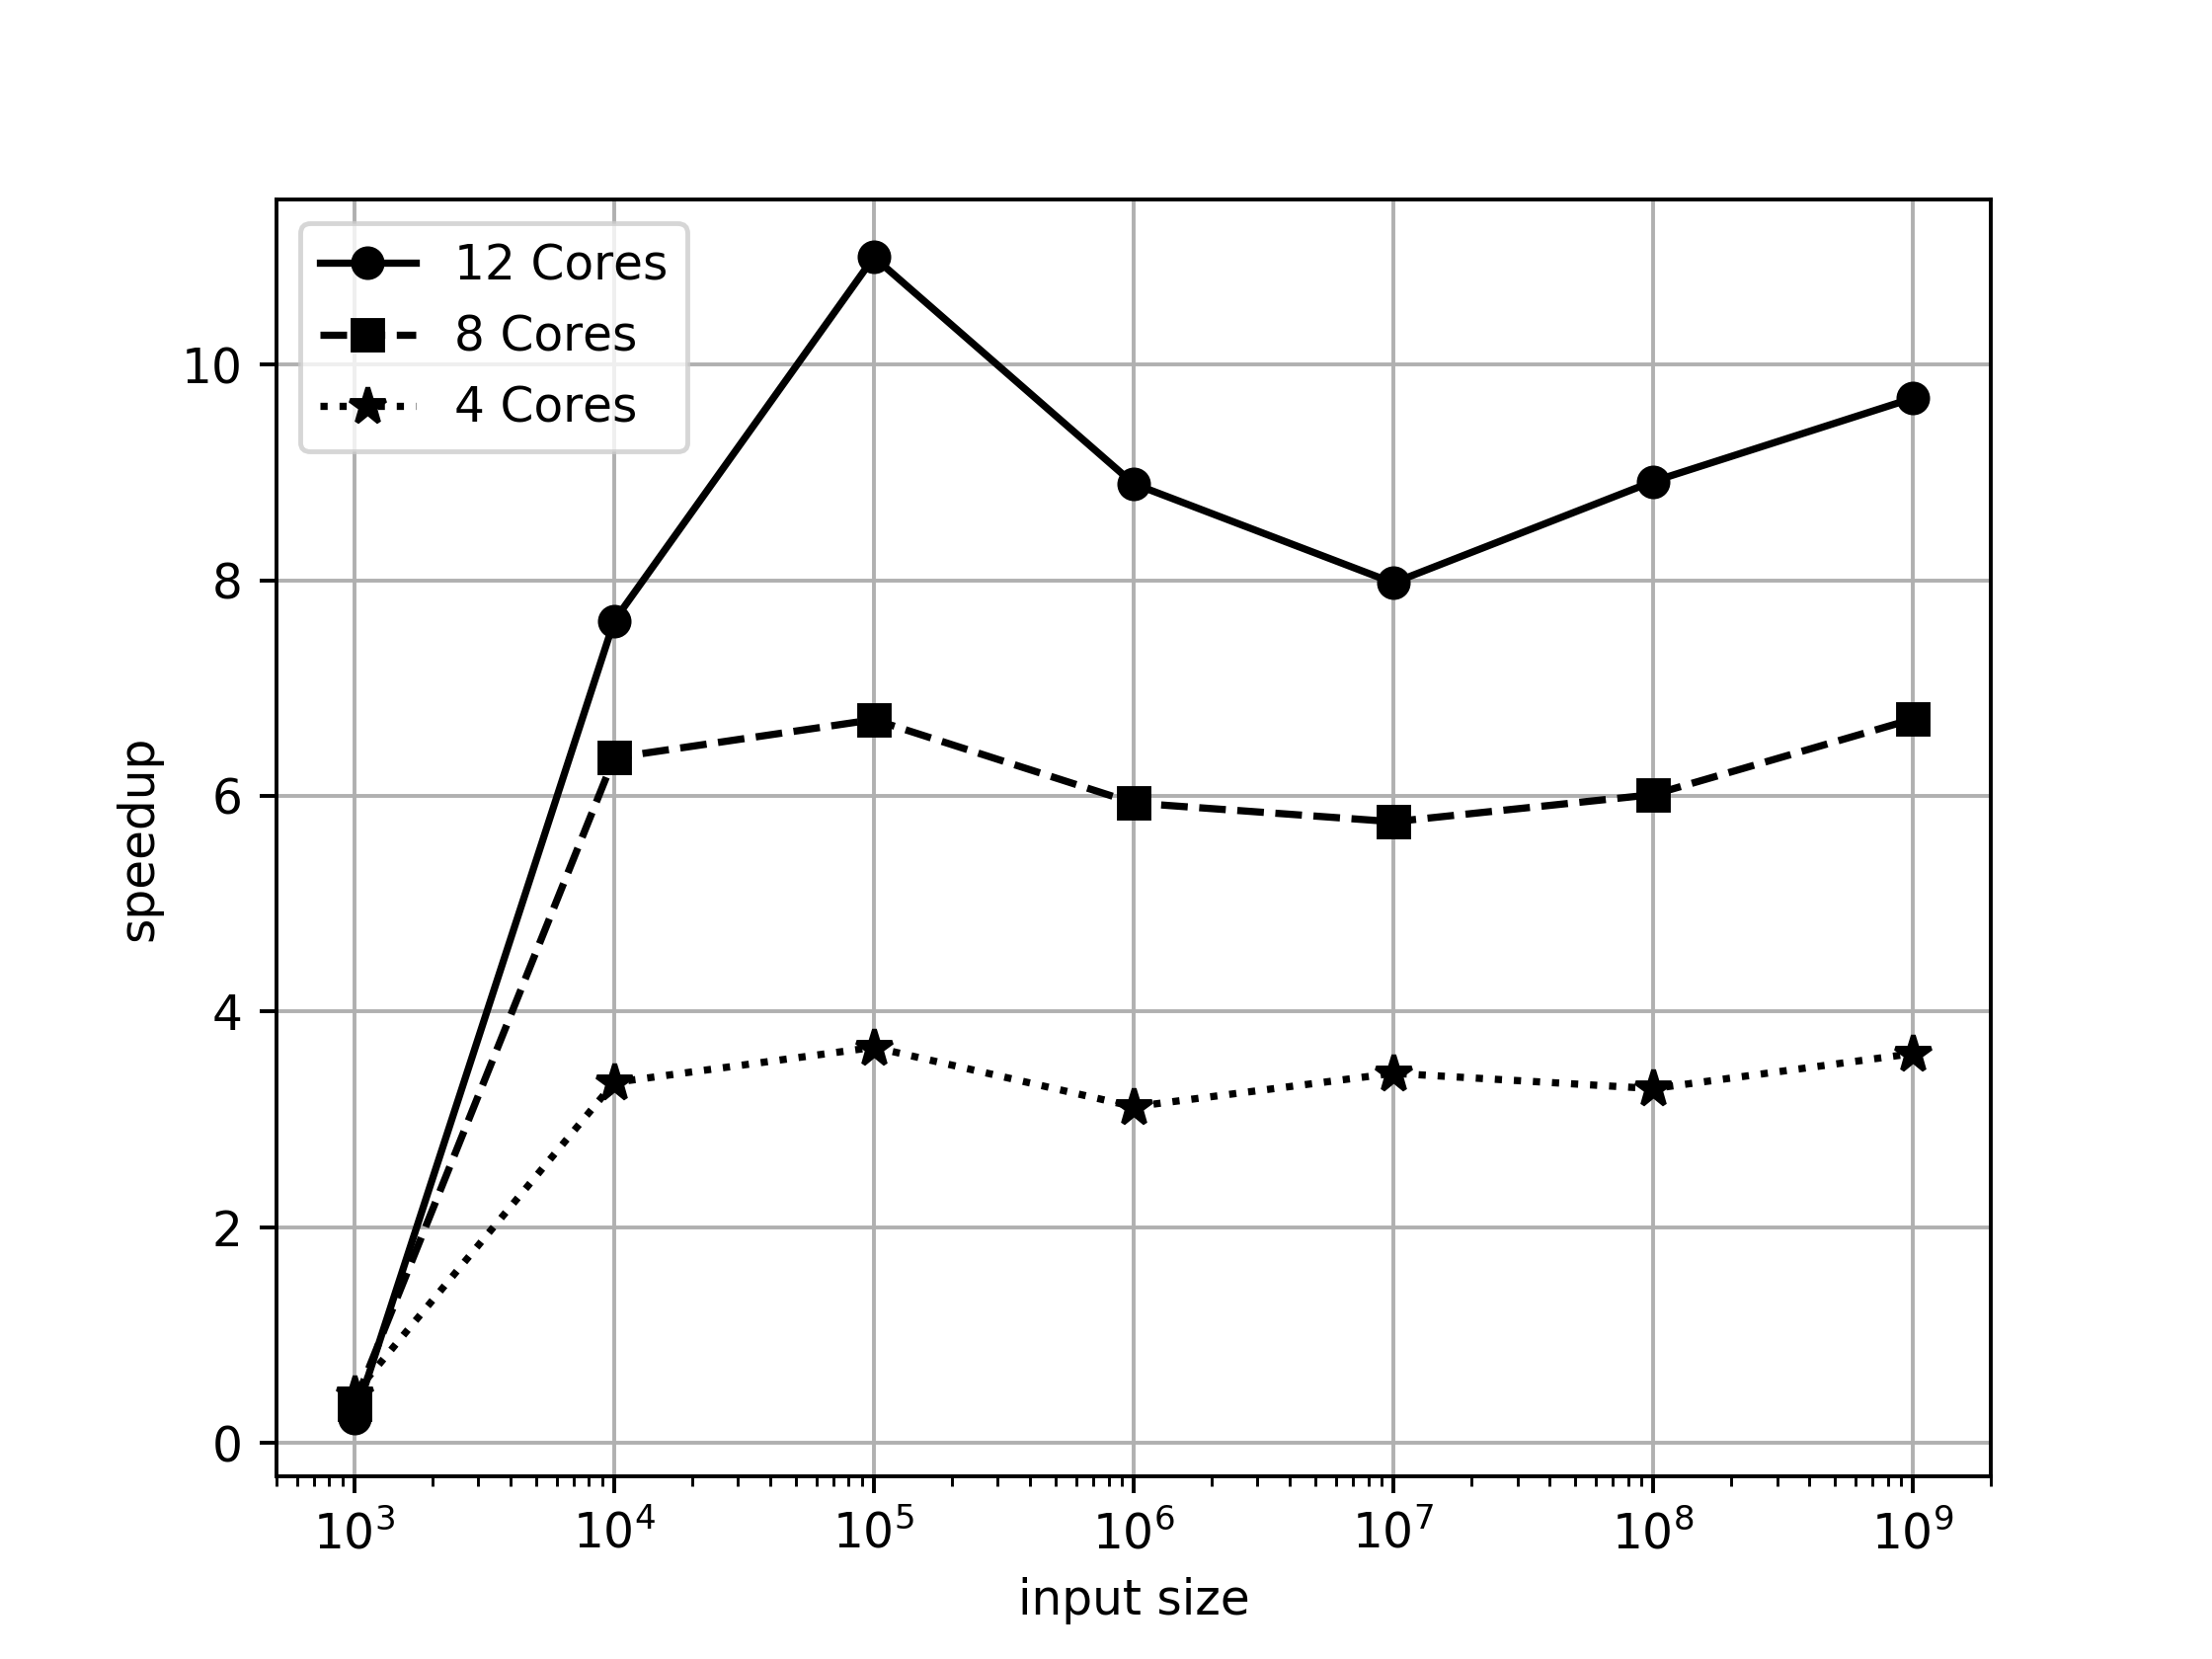
\includegraphics[width=\textwidth]{pispeedup_size.png}
        \caption{speedup vs input size}
        \label{fig:q1p10}
    \end{figure}
    \textbf{Figure \ref{fig:q1p3}} shows the variation of speedup with problem size. Notice that speedup first increases till problem size becomes $10^5$ and then remains the same more or less.
    
    Initially as the input size is small, the parallel overhead dominates over the time saved by parallelizing the code. As the problem size increases, the compute time becomes larger , whereas the parallel overhead remains more or less the same. Hence more compute time is saved by parallelizing the code thereby giving us greater and greater speedup.
    
    Unlike the previous question, there is not much memory access required here. Hence for large input sizes, speedup remains roughly the same.
    \newpage
    \subsection{Speedup vs number of cores}
    \begin{figure}[H]
        \centering
        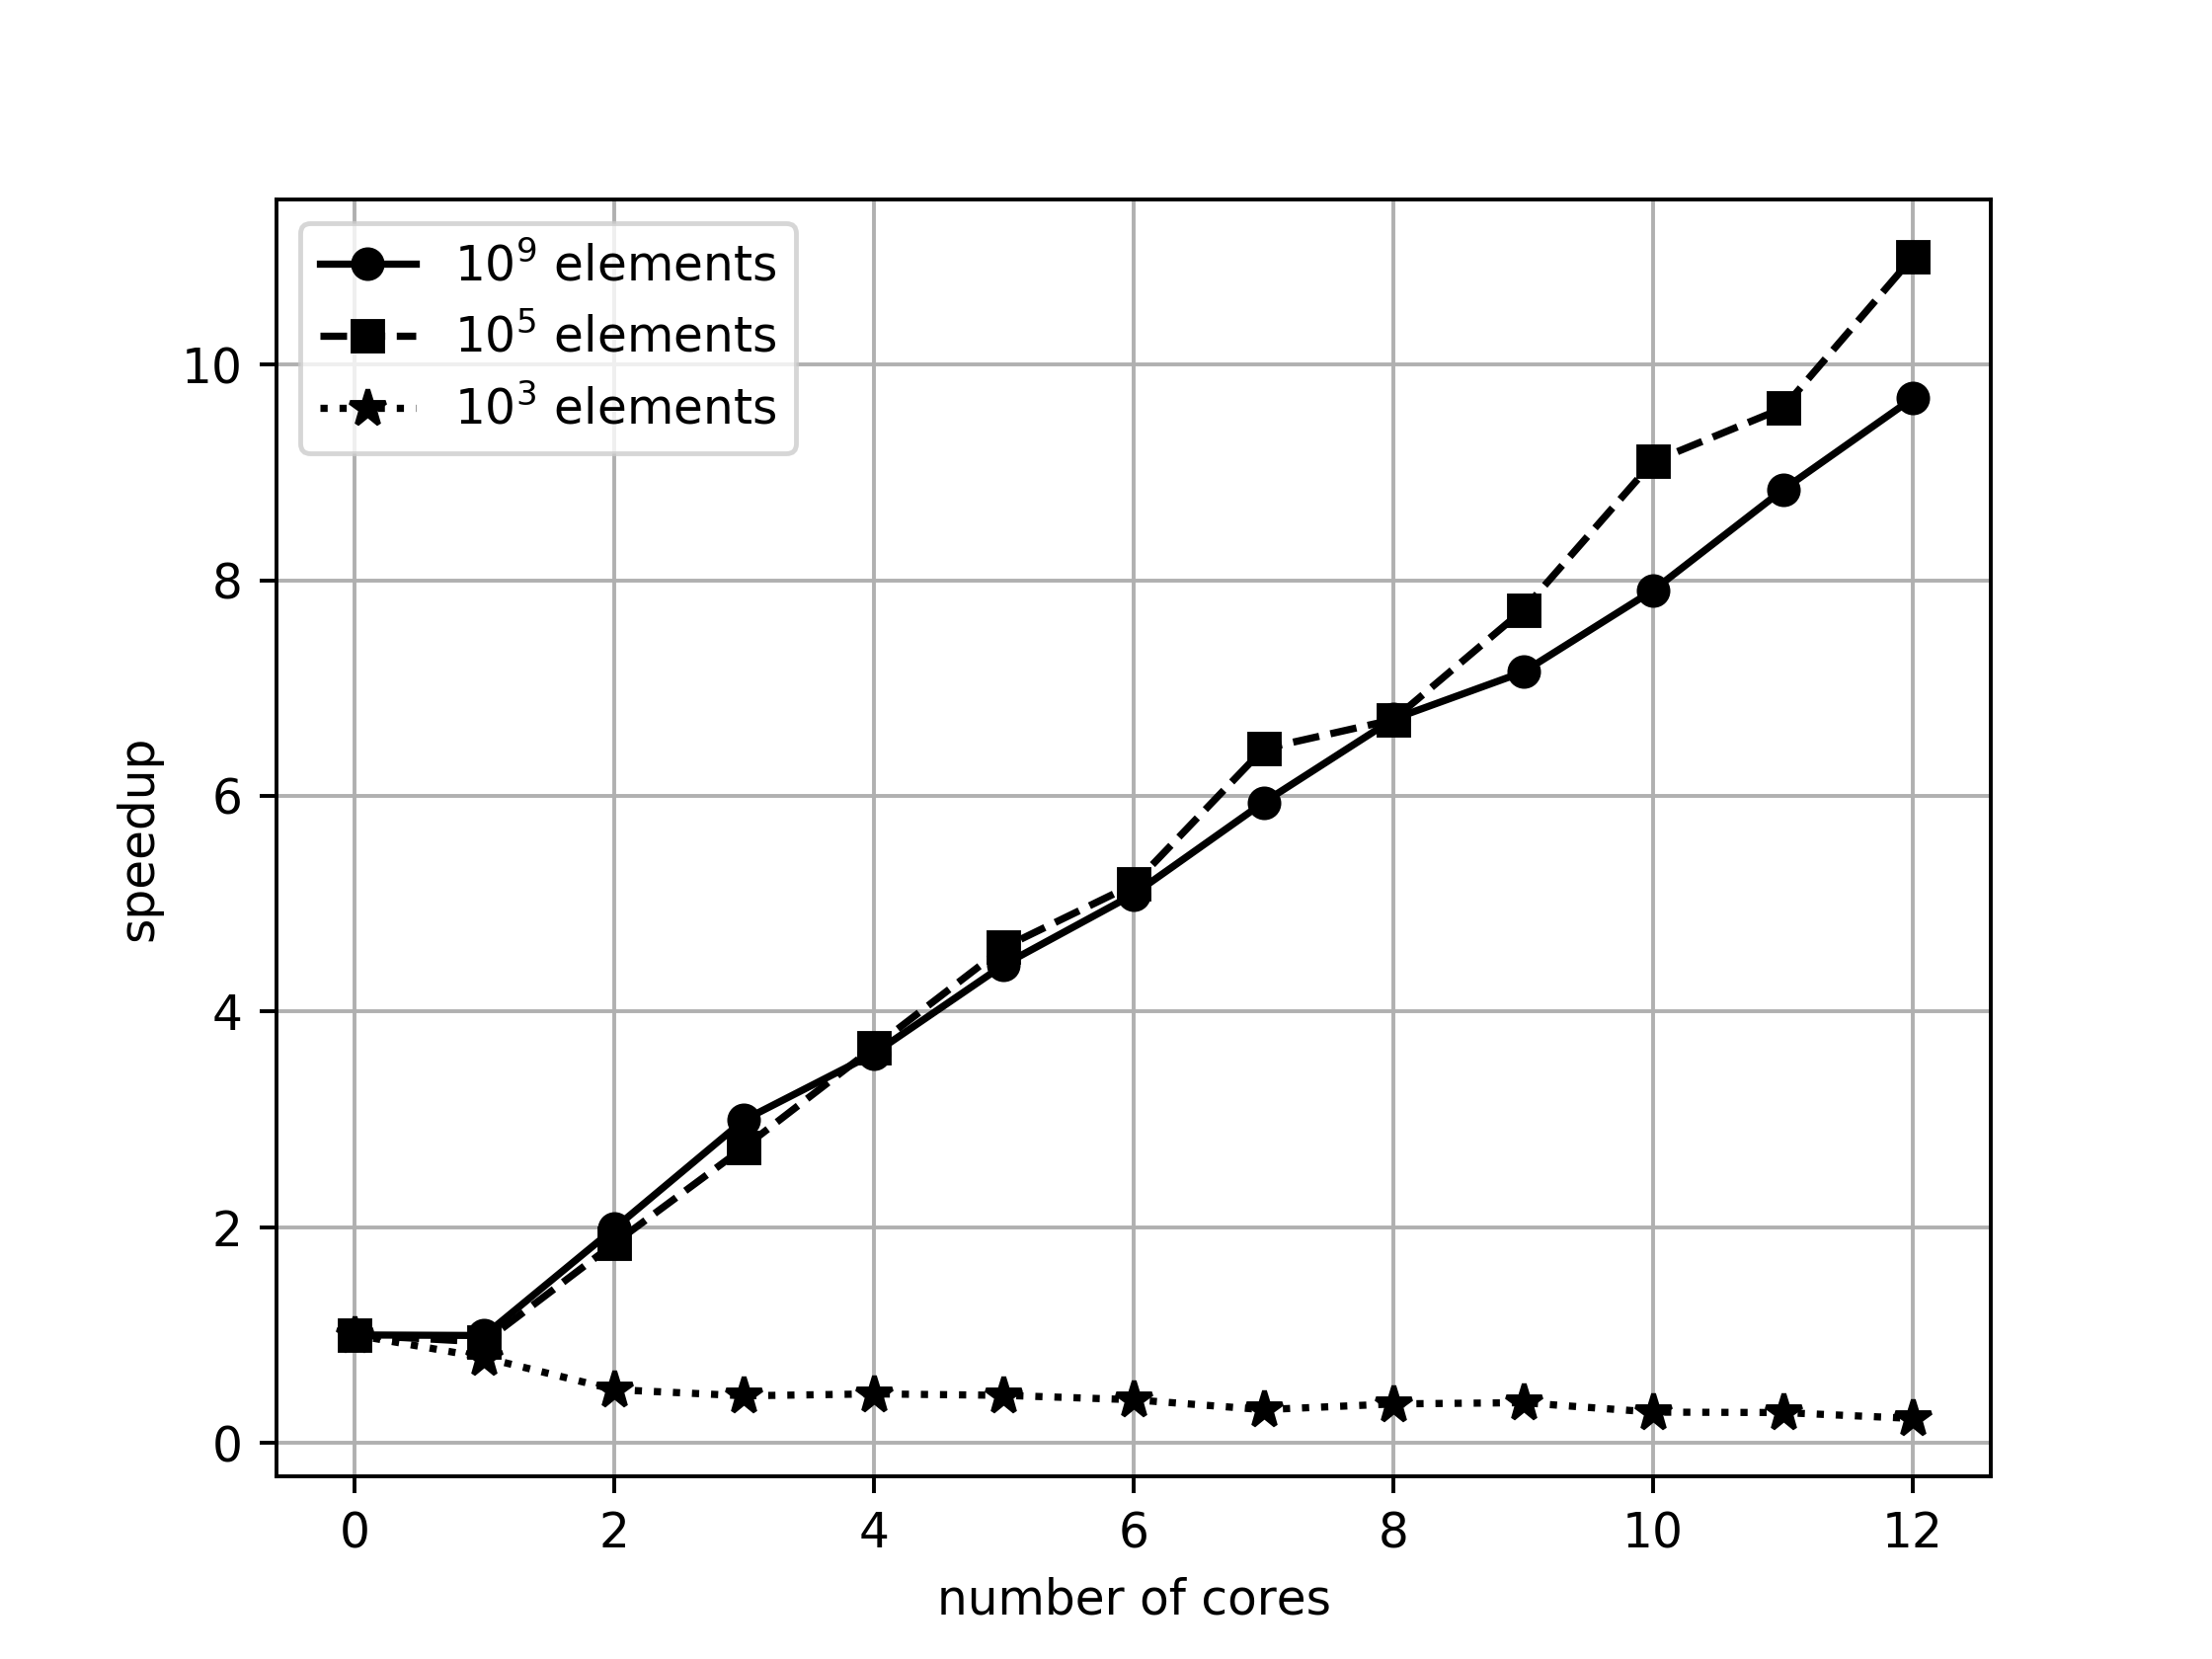
\includegraphics[width=\textwidth]{pispeedup_cores.png}
        \caption{speedup vs number of cores}
        \label{fig:q1p10}
    \end{figure}
    \textbf{Figure \ref{fig:q1p10}} shows the variation of speedup with the number of cores for different problem sizes. 2 notable patterns can be seen here.
    
    When the problem size is small(of the order of $10^3$), increasing the number of cores just adds more parallel overhead because of increased inter-processor synchronization and communication. This is not compensated by the time saved in parallelization since the compute time is already very low incase of the serial code.
    
    For large problem sizes, the case is opposite. Adding a new processor increases the speedup. This is because the compute time is inversely proportional to the number of processors. For large input sizes, the compute time is very high. So even though the parallel overhead increases slightly, a huge amount of time is saved by adding one extra processor. However note that the marginal gain in speedup by addition of 1 processor remains the same as the number of processors increase. Thus speedup does not follow the \textbf{law of diminishing marginal returns} in this problem.  Hence this problem is \textbf{highly scalable} since speedup remains the same.
    \newpage
    \subsection{Convergence to $\pi$}
    On serial execution, the algorithm takes 32.439 seconds to calculate the value of $\pi$ as 3.1416. On 12 cores the parallel algorithm gives the same accuracy in $3.36$ seconds. Giving a speedup of roughly 10.
\end{document}